\documentclass{ltxdockit}
\usepackage{btxdockit}
\usepackage[utf8]{inputenc}
\usepackage[french]{babel}
\usepackage[babel]{csquotes}
\usepackage{tabularx}
\usepackage{longtable}
\usepackage{booktabs}
\usepackage{shortvrb}
\usepackage{pifont}

\MakeOuterQuote{"}
\MakeAutoQuote*{<}{>}
\MakeShortVerb{\|}

\rcsid{$Id: droit-fr.tex,v 1.1 2016/20/02 16:00:00 ydsp stable $}

\newcommand*{\biber}{Biber\xspace}
\newcommand*{\biblatex}{Biblatex\xspace}

\newcommand*{\classname}{droit-fr\xspace}
\newcommand*{\bibstylename}{droit-fr\xspace}

\makeatletter
\renewenvironment*{typelist}
  {\list{}{%
     \setlength{\labelwidth}{\marglistwidth}%
     \setlength{\labelsep}{\marglistsep}%
     \setlength{\leftmargin}{0pt}%
     \renewcommand*{\makelabel}[1]{\hss\marglistfont##1}}%
   \def\typeitem##1{%
     \item[{##1}]%
     \ltd@pdfbookmark{##1}{##1}}%
   \def\reqitem{%
     \par\begingroup\itemsep0.5\itemsep\item
     Requis: \btd@fieldloop}
   \def\optitem{%
     \par\begingroup\itemsep0.5\itemsep\item
     Optionnel: \btd@fieldloop}}
  {\endlist}

\renewenvironment*{fieldlist}
  {\list{}{%
     \setlength{\labelwidth}{\marglistwidth}%
     \setlength{\labelsep}{\marglistsep}%
     \setlength{\leftmargin}{0pt}%
     \renewcommand*{\makelabel}[1]{\hss\marglistfont##1}}%
   \def\fielditem##1##2{%
     \item[##1]%
     \ltd@pdfbookmark{##1}{##1}%
     champ (##2)\par\nobreak
     \vspace{\itemsep}}%
   \def\listitem##1##2{%
     \item[##1]%
     \ltd@pdfbookmark{##1}{##1}%
     liste (##2)\par\nobreak
     \vspace{\itemsep}}}
  {\endlist}
\makeatother

\titlepage{%
  title={\LaTeX\ appliqué au droit français},
  subtitle={Des outils adaptés à la rédaction de thèses en droit},
  author={Yves de Saint-Pern},
  email={yves.desaintpern@gmail.com},
  revision={\rcsrevision},
  date={\rcstoday}}

\hypersetup{%
  pdftitle={\latex appliqué au droit français},
%  pdfsubject={},
  pdfauthor={Yves de Saint-Pern}}

% tables

\newcolumntype{H}{>{\sffamily\bfseries\spotcolor}l}
\newcolumntype{L}{>{\raggedright\let\\=\tabularnewline}p}
\newcolumntype{R}{>{\raggedleft\let\\=\tabularnewline}p}
\newcolumntype{C}{>{\centering\let\\=\tabularnewline}p}
\newcolumntype{V}{>{\raggedright\let\\=\tabularnewline\ttfamily}p}

\newcommand*{\sorttablesetup}{%
  \tablesetup
  \ttfamily
  \def\new{\makebox[1.25em][r]{\ensuremath\rightarrow}\,}%
  \def\alt{\par\makebox[1.25em][r]{\ensuremath\hookrightarrow}\,}%
  \def\note##1{\textrm{##1}}}

\newcommand{\tickmarkyes}{\Pisymbol{psy}{183}}
\newcommand{\tickmarkno}{\textendash}
\providecommand*{\textln}[1]{#1}
\providecommand*{\lnstyle}{}

% markup and misc

\setcounter{secnumdepth}{4}

\makeatletter

\newenvironment{nameparts}
  {\trivlist\item
   \tabular{@{}ll@{}}}
  {\endtabular\endtrivlist}

\newenvironment{namedelims}
  {\trivlist\item
   \tabularx{\textwidth}{@{}c@{=}l>{\raggedright\let\\=\tabularnewline}X@{}}}
  {\endtabularx\endtrivlist}

\newenvironment{namesample}
  {\def\delim##1##2{\@delim{##1}{\normalfont\tiny\bfseries##2}}%
   \def\@delim##1##2{{%
     \setbox\@tempboxa\hbox{##1}%
     \@tempdima=\wd\@tempboxa
     \wd\@tempboxa=\z@
     \box\@tempboxa
     \begingroup\spotcolor
     \setbox\@tempboxa\hb@xt@\@tempdima{\hss##2\hss}%
     \vrule\lower1.25ex\box\@tempboxa
     \endgroup}}%
   \ttfamily\trivlist
   \setlength\itemsep{0.5\baselineskip}}
  {\endtrivlist}

\makeatother

\begin{document}

\printtitlepage
\tableofcontents
\listoftables

\section{Introduction}
\label{int}

\subsection{Des limites de l'informatique en droit français}

Beaucoup d'auteurs ont déjà utilisé l'un des deux logiciels de traitement de texte les plus courants, Microsoft Word ou OpenOffice Writer. Relativement faciles à prendre en main, ces logiciels généralistes répondent à un grand nombre de besoins, mais ne répondent pas aux exigences d'ouvrages complexes et de grande taille.

Le mémoire de thèse en est un exemple. Dans ce type d'ouvrage de plusieurs centaines de pages, la bibliographie tient une place très importante et exige une grande rigueur de présentation. Face à ce défi, les traitements de texte de base précités ne sont pas d'un grand secours, si bien que de nombreux rédacteurs perdent un temps précieux à recopier manuellement des lignes de références bibliographiques pour obtenir un résultat souvent médiocre. 

Il existe des logiciels qui facilitent ce processus de manière significative. Toutefois, les codes juridiques de présentation d'une bibliographie s'avèrent exotiques: jurisprudence, lois, mélanges et autres ouvrages juridiques doivent être cités selon des règles que la plupart des logiciels en bibliographie ne prennent pas en charge. Les doctorants en droit n'ont donc d'autre choix que de consacrer une part très substantielle de leur temps à la mise en forme de leur document, et ce au détriment du fond.

\subsection{Qu'est-ce que \latex ?}

Les traitements de texte grand public proposent une interface intuitive: l’utilisateur voit s'afficher en temps réel le rendu final de son document\footnote{On parle dans ce cas d'interface WYSIWYG, acronyme de "What you see is what you get".}. 
Le traitement de texte \latex propose une approche radicalement différente: séparer le fond et la forme. La rédaction s'effectue alors en deux étapes:
\begin{enumerate}

\item l'auteur travaille d'abord sur un document "source" (d'extension \file{.tex}), dans lequel il utilise des balises (rappelant le HTML) afin de structurer son document, formater le texte, etc.

\item le rendu final est obtenu par un processus dit de "compilation" au cours duquel le contenu du fichier source est analysé puis transformé en fichier PDF (ou autre).

\end{enumerate}

Il ne faut pas se leurrer: \latex demande un temps d'adaptation. L'utilisation des commandes de mise en forme n'est pas très complexe mais déroutante pour les personnes habituées à travailler sur des logiciels comme Word, où le rendu d'un document leur est présenté immédiatement; sans compter que des erreurs peuvent être détectées à la compilation.

Toutefois, les atouts de \latex sont nombreux:

\begin{enumerate}

\item Le principe fondamental est la séparation du fond et de la forme. Pendant la rédaction, l'auteur ne se préocupe \emph{jamais} du rendu final, mais reste focalisé sur son propos ce qui permet de lui faire gagner beaucoup de temps. \latex est donc particulièrement avantageux lorsque le document a rédiger est très gros, car dans ce cas, le temps d'apprentissage du langage devient négligeable par rapport à la durée totale de rédaction.

\item la gestion automatisée de la bibliographie: citer un ouvrage est une opération très simple dans un document \latex. Les règles complexes de présentation des citations sont gérées atomatiquement au moment de la compilation.

\item d'autres outils automatiques sont proposés dans \latex: la création d'index, de glossaire, de table des matières active, de liens Internet actifs.

\item \latex est gratuit, et compatible avec Windows, Mac et Linux.

\end{enumerate}

\subsection{\latex en droit français, est-ce possible ?}

\latex a déjà fait ses preuves dans le monde académique. Il est aujourd'hui le traitement de texte de prédiléction des doctorants en sciences mais aussi de nombreuses revues scientifiques de renom. Toutefois, \latex peine à s'imposer en sciences humaines, et ce pour plusieurs raisons: la caractère non-intuitif de cet outil est probablement rebutant pour des personnes peu portées sur la technique et l'informatique en général; d'autre part, il n'existe pas de règle universelle de présentation en droit français, seulement des usages.

Certaines universités en droit autorisent maintenant la rédaction de thèse sous \latex. Toutefois, aucune feuille de style n'est proposée et les étudiants aventureux se retrouvent généralement perdus face aux contraintes techniques et au manque de formation.

Ce document a pour objectif de répondre à leur besoin, au moyen de deux extensions spécifiquement prévues pour le droit français vont être présentées dans ce document:
\begin{enumerate}
\item une classe \latex de thèse en droit (\secref{classe});
\item un style bibliographique pour les ouvrages juridiques (\secref{bibliographie}).
\end{enumerate}
Un exemple pratique utilisant ces deux extensions sera exposé dans \secref{template}. Enfin, des recommandations, astuces et notes diverses feront l'objet d'une dernière partie (\secref{astuces}).

\subsection{Comment utiliser cette documentation}

Avant d'aller plus loin, des connaissances de base en \latex sont nécessaires. La présente documentation n'a en effet pas pour but de revenir sur les fondamentaux de \latex, qui font l'objet de nombreux tutoriaux, site et spécifications abondantes sur Internet. En voici quelques-uns:
\begin{itemize}
\item Le site de l'ENS propose un tutoriel\fnurl{http://www.tuteurs.ens.fr/logiciels/latex} un peu austère mais complet et pédagogue (en français)
\item un guide officiel présenté sous la forme d'un wiki\fnurl{http://fr.wikibooks.org/wiki/LaTeX}, très bien fait. Une section \href{http://fr.wikibooks.org/wiki/LaTeX/Vade_mecum#Structuration_du_document}{vade mecum} peut servir de mémo des commandes les plus courantes.
\end{itemize}

Mais l'ouvrage introductif le plus pertinent pour les étudiants de droit est certainement \enquote{Latex appliqué aux sciences humaines}, écrit par Maieul Rouquette\fnurl{http://geekographie.maieul.net/Xe-LaTeX-applique-aux-sciences}. Cet ouvrage présente plusieurs avantages: il est particulièrement adapté, comme son titre l'indique, à des personnes qui ne viennent pas du monde des sciences dures; il est par ailleurs lisible, et très complet.

\section{\sty{\classname}, une classe \latex pour les thèses en droit}
\label{classe}

La classe \sty{\classname} est adaptée à des contraintes inhérentes aux mémoires de thèses en droit français. 
En voici quelques caractéristiques générales:
\begin{itemize}
\item Page de titre adaptable
%\item Double table des matières (sommaire et version longue)
\item En-têtes et pieds-de-pages automatiques
\item 10 niveaux hiérarchiques disponibles
\item Paragraphes numérotés (versets)
\item Index par numéro de versets
\end{itemize}

\subsection{Installation}

La classe \sty{\classname} est définie dans le fichier \file{\classname.cls}. Cette classe doit être placée dans le répertoire de travail ou bien dans un répertoire connu de la distribution \latex installée.

Les packages \latex suivants doivent également avoir été installés:
\begin{itemize}
\item \sty{memoir}: classe de laquelle \sty{\classname} est dérivée.
\item \sty{csquotes}: pour la gestion des guillemets français
\item \sty{hyperref}: support des hyperliens PDF
\item \sty{bookmark}: support des signets PDF
\item \sty{engrec}: support des caractères grecs
\end{itemize}

\subsection{Options}

Cette section liste les options spécifiques à la classe \sty{\classname}.

\begin{optionlist}

\boolitem[false]{footnotereset}

Cette option contrôle le mode de numérotation des notes de bas de page. Lorsque cette option est passée avec la valeur \texttt{false}, les notes de bas de pages sont numérotées de manière continue tout le long du document. La valeur \texttt{true} permet de renuméroter les notes à partir de 1 pour chaque nouvelle page.

\boolitem[true]{versetitle}

Cette option contrôle l'affichage des titres de versets (voir \secref{versets}). Lorsque cette option est passée avec la valeur \texttt{false}, les titres passés en paramètre de la commande \cmd{verset} sont ignorés à la compilation; la commande \cmd{verset} se borne alors à numéroter un paragraphe. La valeur \texttt{true} affiche normalement les titres, comme le font les commandes listées en section \secref{sections}.


\end{optionlist}

\subsection{Page de titre}

\begin{ltxsyntax}

\cmditem{university}{université}
\cmditem{school}{école}
\cmditem{speciality}{spécialité}
\cmditem{approvaldate}{date}

Ces commandes renseignent sur l'université, l'école doctorante, la spécialité de la thèse et la date de soutenance.

\cmditem{director}{civilité}{prénom}{nom}{poste}
\cmditem{reportera}{civilité}{prénom}{nom}{poste}
\cmditem{reporterb}{civilité}{prénom}{nom}{poste}
\cmditem{membera}{civilité}{prénom}{nom}{poste}
\cmditem{memberb}{civilité}{prénom}{nom}{poste}

Ces commandes renseignent les cinq membres du jury: le directeur de thèse, les deux rapporteurs et les deux examinateurs. 4 arguments sont à remplir, la civilité, le prénom, le nom de famille et enfin l'intitulé complet de poste.

\cmditem{maketitlepage}

Imprime la page de titre à la position courante.

\end{ltxsyntax}

\subsection{Niveaux hiérarchiques}
\label{sections}

En droit français, tout niveau hiérarchique est subdivisé de manière binaire: une partie est divisée en deux titres, chacun d'entre eux en deux chapitres et ainsi de suite. Pour cette raison, le nombre de niveaux hiérarchiques proposés par défaut dans les classes de base de \latex s'avère insuffisant pour les besoins d'une thèse en droit.

La classe \sty{memoir} (de laquelle dérive la classe \sty{\classname}) offre non seulement une nombre de niveaux  plus élevé mais aussi des outils permettant d'en créer de nouveaux, allant en-deçà du \cmd{subsubparapgraph}\footnote{Pour plus de précisions, voir la documentation de la classe memoir et plus précisément la commande \cmd{newlist}.}. Toutes les commandes de cette classe sont donc utilisables, mais leur nom peut prêter à confusion. Aussi, sont également proposés des alias francisés, plus intuitifs dans un contexte de droit français.

\begin{table}
\tablesetup
\begin{tabularx}{\textwidth}{@{}p{100pt}@{}p{100pt}@{}>{\ttfamily}X@{}}
\toprule
\multicolumn{1}{@{}H}{Commande francisée} &
\multicolumn{1}{@{}H}{Commande d'origine} &
\multicolumn{1}{@{}H}{Niveau} \\
\cmidrule(r){1-1}\cmidrule(r){2-2}\cmidrule{3-3}
\cmd{partie} & \cmd{book} & -2 \\
\cmd{titre}  & \cmd{part} & -1 \\
\cmd{chapitre}  & \cmd{chapter} & 0 \\
\cmd{section} &  \cmd{section} & 1 \\
\cmd{paragraphe}  & \cmd{subsection} & 2 \\
\cmd{souspara} &  \cmd{subsubsection} & 3 \\
\cmd{alinea} &  \cmd{paragraph} & 4 \\
\cmd{sousalinea}  & \cmd{subparagraph} & 5 \\
\cmd{point} &  \cmd{subsubparagraph} & 6 \\
\cmd{souspoint}  & -- & 7 \\
\cmd{verset}  & -- & 8 \\
\bottomrule
\end{tabularx}
\caption{Niveaux de hiérarchie disponibles}
\label{sectionlevels}
\end{table}

La convention de nommage des niveaux hiérarchiques choisie ici correspond aux usages les plus courants en droit français. Toutefois, les niveaux intermédiaires suivants ne sont pas pris en charge:
\begin{itemize}
\item les "sous-titres", entre les titres et les chapitres
\item les "sous-sections", entre les sections et les paragraphes.
\end{itemize}
Le rendu visuel de chaque niveau a été choisi de manière arbitraire.

\subsection{Versets}
\label{versets}

Il est d'usage en droit français de numéroter des blocs de paragraphe, notamment dans les thèses. Ces paragraphes numérotés seront dans la suite appelés "versets".

\begin{ltxsyntax}

\cmditem{verset}{titre}

La commande \cmd{verset} peut être considérée comme une commande de section de faible niveau, mais présente des particularités: son compteur n'est jamais remis à zéro et peut être utilisée à n'importe quel niveau hiérarchique; de plus il est possible d'en laisser le titre vide.

Un point final est automatiquement ajouté à la fin du titre du verset, si l'argument passé à la commande n'est pas déjà terminé par l'un des caractère de ponctuation suivants: point (.), point d'exclamation (!), point d'interrogation (?) ou trois petits points (\ldots). Ce mécanisme dispense donc le rédacteur de systématiquement terminer chaque libellé de verset par un tel point.

\cmditem{vref}{label}

Dans la mesure où la commande \cmd{verset} est une commande de section conventionnelle\footnote{C'est-à-dire qu'elle se fonde sur la commande interne \cmd{\\@startsection}.}, les mécanismes habituels de références croisées sont applicables aux versets \footnote{Typiquement, la commande \cmd{label} pour créer une référence croisée, commande \cmd{ref} pour créer un lien vers une référence croisée.}.

La commande \cmd{vref} propose un rendu spécial pour les versets.
\begin{itemize}
\item Lorsque le verset désigné par \texttt{label} se trouve à une page antérieure à la page courante, est imprimé le terme "supra" en italiques, suivi du numéro de verset, suivi du numéro de page auquel débute le verset.

\item Lorsque le verset désigné par \texttt{label} se trouve à une page antérieure à la page courante, est imprimé le terme "infra" en italiques, suivi du numéro de verset, suivi du numéro de page auquel débute le verset.

\item Lorsque le verset désigné par \texttt{label} se trouve à une page antérieure à la page courante, est imprimé le terme "supra", suivi du numéro de verset, suivi du numéro de page correspondant.
\end{itemize}

Supposons par exemple que l'on invoque \cmd{vref} depuis la page 100, que le paramètre de la commande désigne une référence croisée déclarée au moyen de \cmd{label} à la page 50 et à l'intérieur d'un verset ayant pour numéro 27. 
Le rendu sera alors:

\begin{quote}
\emph{supra}, n\textsuperscript{o}27, p. 50
\end{quote}

\cmditem{fvref}{label}

Une variante de la commande \cmd{vref}, qui renvoie à une note de page de page.

\end{ltxsyntax}

\subsection{En-têtes et pied-de-pages}
\label{entete}

L'en-tête des pages impaires contient le titre de la division hiérarchique courante (partie, titre, chapitre, section ou paragraphe). Depuis une subdivision de niveau inférieur (sous-paragraphe, etc), le paragraphe courant est affiché dans l'en-tête.

L'en-tête des pages paires contient le titre de l'ouvrage (passé à la commande \cmd{title}).

Le pied de page contient le numéro de la page courante centré.

À noter que l'en-tête et le pied-de-page sont désactivés dans le cas d'une page blanche.

\subsection{Index}
\label{index}

L'index de base proposé par \latex référence des termes à l'aide de numéros de page. Deux index supplémentaires, utilisant des numéros de verset, sont proposés par la classe \sty{droit-fr}.

\subsubsection{Index de base par versets}

\begin{ltxsyntax}

\cmditem{makeindexv}

Génère un fichier d'index par versets. À invoquer dans le préambule du document, similairement à la commande \cmd{makeindex} fournie par \latex.

\cmditem{indexv}{mot}

Ajoute un mot-clé au fichier d'index par versets. Cette commande est identique à la commande de base \cmd{index} fournie par \latex à ceci près que le référencement est effectué par versets et non par pages. Toutes les paramètres optionnels de la commande \cmd{index} sont applicables.

\cmditem{printindexv}

Imprime l'index complet par versets à la position courante. Bien entendu, la commande \cmd{makeindexv} doit avoir été invoquée dans le préambule du document.

\end{ltxsyntax}

\subsubsection{Index d'auteurs par versets}
\label{indexauteurs}

L'index d'auteurs est un index spécifiquement dédié, comme son nom l'indique, aux auteurs cités dans le document. Il référence des numéros de versets, comme l'index de base.

\begin{ltxsyntax}

\cmditem{makeindexa}

Génère un fichier d'index d'auteurs par versets. À invoquer dans le préambule du document, similairement à la commande \cmd{makeindex} fournie par \latex.

\cmditem{indexa}{mot}

Ajoute un mot-clé au fichier d'index d'auteurs par versets. Cette commande est identique à la commande de base \cmd{index} fournie par \latex à ceci près que le référencement est effectué par versets et non par pages. Toutes les paramètres optionnels de la commande \cmd{index} sont applicables.

Cette commande peut être utilisée manuellement dans le document. Toutefois, il est préférable de déléguer ce travail d'indexation au package biblatex moyennant l'activation de l'option \texttt{indexing=cite}, et de l'ajout d'une instruction spéciale dans le préambule du document permettant à biblatex d'utiliser en interne cette commande \cmd{indexa} (voir à ce propos le préambule du template de la section \ref{template}). L'index par auteur est ainsi entièrement constitué de tous les auteurs cités via la commande \cmd{cite}.

\cmditem{printindexa}

Imprime l'index d'auteurs à la position courante. La commande \cmd{makeindexa} doit avoir été invoquée dans le préambule du document.

\end{ltxsyntax}



%%%%%%%%%%%%%%%%%%%%%%%%%%%%%%%%%%%%%%%%%%%%%%%%%%%%%%%%%%%%%%%%%%%%%

\section{\sty{\bibstylename}, un style de bibliographie juridique}
\label{bibliographie}

\subsection{Installation}

Le style \sty{\bibstylename} est composé de deux fichiers, \file{droit-fr.bbx} et \file{droit-fr.cbx} contenant respectivement les réglages relatifs à la bibliographie et aux citations. Ces deux fichiers doivent être placés dans un répertoire reconnu par la distribution \latex installée ou bien dans le répertoire de travail courant.

Le package \biblatex est nécessaire. Il doit être invoqué dans le préambule du document de travail à l'aide de la commande \cmd{usepackage} (voir \secref{template} pour un exemple concret).

Le programme \biber doit également être installé. Il faut l'utiliser en lieu et place du vénérable \bibtex au moment de la compilation (voir \secref{compilation} pour plus détails concernant la compilation).

\textbf{Attention, il est nécessaire d'installer une version suffisamment récente de \biblatex (3.0 minimum), sous peine d'erreurs à la compilation}. De plus, la version de \biber doit être compatible avec la version de \biblatex installée . Une solution simple pour résoudre ces deux problèmes d'un coup est probablement d'installer les dernières versions proposées par le gestionnaire de packages de la distribution \latex utilisée.

\subsection{Options}
\label{biboptions}

Les options suivantes sont utilisables lors du chargement du package \biblatex au moyen de la commande \cmd{usepackage}, dans le préambule du document.

\begin{optionlist}

\optitem[permit]{citepages}{\opt{permit}, \opt{suppress}, \opt{omit}, \opt{separate}}

Cette option contrôle le traitement du champ \bibfield{pages} dans les citations. Lorsqu'une entrée avec un champ \bibfield{pages} renseigné est citée pour la première fois, et que la postnote est un numéro ou intervalle de pages, la citation peut comporter plusieurs informations de pages concurrentes.

L'option \texttt{citepages} propose différentes stratégies de présentation, déjà proposées dans d'autres styles\footnote{Les styles \texttt{verbose-ibid}, \texttt{verbose-trad} en particulier.}. Les rendus respectifs de ces stratégies vont être exposés au regard de la séquence d'exemple suivante:

\begin{ltxexample}
\cite{cle}
\cite[une note]{cle}
\cite[125]{cle}
\end{ltxexample}

Dans cet exemple, une référence bibliographique de clé \bibtex \prm{cle} est cité trois fois; 125 est la postnote et 100-150 la valeur passée au champ \bibfield{pages}.

\begin{valuelist}
\item[permit] Autorise l'affichage simultané des champs \texttt{pages}\slash \texttt{pagetotal} et de la \texttt{postnote}:

\begin{quote}
\textsc{Auteur}, \emph{titre}, p. 100-150. 

\textsc{Auteur}, \emph{titre}, p. 100-150, une note.

\textsc{Auteur}, \emph{titre}, p. 100-150, p. 125.
\end{quote}
%
\item[suppress] Supprime inconditionnellement les champs \texttt{pages}\slash \texttt{pagetotal} dans les citations, quelque soit la \texttt{postnote}.

\begin{quote}
\textsc{Auteur}, \emph{titre}. 

\textsc{Auteur}, \emph{titre}, une note.

\textsc{Auteur}, \emph{titre}, p. 125.
\end{quote}
%
\item[omit] Supprime les champs \texttt{pages}\slash
\texttt{pagetotal} seulement dans le troisième cas. Ils sont malgré tout imprimés si la \texttt{postnote} est vide ou n'est pas un chiffre ni un intervalle (voir \secref{use_cav_pag} à ce sujet):

\begin{quote}
\textsc{Auteur}, \emph{titre}, p. 100-150. 

\textsc{Auteur}, \emph{titre}, p. 100-150, une note.

\textsc{Auteur}, \emph{titre}, p. 125.
\end{quote}
%
\item[separate] Sépare les champs \texttt{pages}\slash
\texttt{pagetotal} de la \texttt{postnote} dans le troisième cas:

\begin{quote}
\textsc{Auteur}, \emph{titre}, p. 100-150. 

\textsc{Auteur}, \emph{titre}, p. 100-150, une note.

\textsc{Auteur}, \emph{titre}, p. 100-150, spéc. p. 125.
\end{quote}
%
On notera que le mot séparateur \enquote{spéc.} est spécifié dans la macro \texttt{thiscite}, qui peut être modifiée.
\end{valuelist}

\optitem[parens]{namestyle}{\opt{parens}, \opt{parensprefix}, \opt{plain}}

Cette option contrôle le rendu des prénoms et des particules de nom de famille dans la bibliographie.

\begin{valuelist}
\item[parens] Valeur par défaut. Le prénom et la particule sont groupés ensemble et mis entre parenthèses après le nom de famille, comme suit:
\begin{quote}
\textsc{Saint-Pern} (Yves de) 
\end{quote}

\item[parensprefix] La particule est positionnée juste après le nom de famille, entre parenthèses; le prénom est positionné après la particule, sans parenthèses, comme suit:
\begin{quote}
\textsc{Saint-Pern} (de), Yves 
\end{quote}

\item[plain] Le prénom et la particule sont groupés ensemble et séparés du nom de famille par une virgule, comme suit:
\begin{quote}
\textsc{Saint-Pern}, Yves de 
\end{quote}
\end{valuelist}

\boolitem[false]{reverseauthors}

Cette option contrôle le rendu du champ \bibfield{author} dans la bibliographie. Lorsque l'option vaut \texttt{true}, alors tous les auteurs listés dans ce champ sont rendus de la même manière, avec le nom de famille en premier suivi du prénom entres parenthèses, comme suit:
\begin{quote}
\textsc{Malaurie} (Philippe), \textsc{Aynès} (Laurent) et \textsc{Stoffel-Munck} (Philippe) 
\end{quote}

Lorsque cette option est positionnée à \texttt{false}, qui est la valeur par défaut, seul le premier auteur est imprimé avec son nom de famille suivi du prénom entre parenthèses; tout auteur supplémentaire est ensuite imprimé avec le prénom suivi du nom de famille, comme suit:
 
\begin{quote}
\textsc{Malaurie} (Philippe), Laurent \textsc{Aynès} et Philippe \textsc{Stoffel-Munck} 
\end{quote}

\boolitem[true]{smartinitials}
Cette option contrôle le mécanisme d'abréviation des prénoms dans les citations. Sont affectés les prénoms contenus dans les champs \bibfield{author} ou \bibfield{editor}. 

Lorsque cette option vaut \texttt{false}, tout prénom est abrégé en son initiale.

Lorsque cette option vaut \texttt{true}, le nombre de lettres du prénom abrégé dépend des premières lettres de ce prénom, conformément à l'usage en France:
\begin{itemize}
\item tout prénom commençant par un digramme (c'est-à-dire deux consonnes formant un seul son) est abrégé en ce digramme. Par exemple, \enquote{Charles} est abrégé en \enquote{Ch.}.
\item tout prénom commençant par un consonne ou un digramme, puis par l ou r, est abrégé en ces premières lettres. Par exemple, \enquote{Claire} est abrégé en \enquote{Cl.}; \enquote{Christian} est abrégé en \enquote{Chr.}.
\item tout autre prénom est abrégé en son initiale.
\end{itemize}

\boolitem[true]{indexnameformat}

Contrôle le rendu des noms de famille dans un index d'auteurs. Lorsque cette option vaut \texttt{true}, chaque nom de famille est imprimé en petites majuscules dans l'index; lorsqu'elle vaut \texttt{false}, chaque nom de famille est imprimé tel quel.

\end{optionlist}

\subsection{Base de données bibliographiques}

On abordera dans cette section les nouveautés apportées par le style \sty{\classname} dans de la base de données bibliographiques: 
\begin{itemize}
\item les types de références (\secref{bib_typ}).
\item les champs affectables à chaque type (\secref{bib_fld}).
\item les chaînes de caractères (\secref{bib_str}).
\item les schémas de tri de réferences (\secref{tri}).
\end{itemize}

\subsubsection{Types de références}
\label{bib_typ}

Les types de références bibliographiques suivants sont décrits dans cette section:
\begin{enumerate}
\item les types \enquote{classiques}, initialement pris en charge par le package \biblatex, mais modifiés par le style bibliographique \sty{\classname} dans le but de répondre à certains usages particuliers en droit, et
\item les types juridiques créés spécifiquement par le style \sty{\classname}.
\end{enumerate}

Tous les autres types de sources pris en charge par le package \biblatex et non modifiés par le style \sty{\classname} ne seront pas abordés ici, étant abondamment décrits dans la documentation de ce package.

Le tableau \ref{bibtypes} récapitule les types à utiliser, en fonction de la référénce.

\begin{table}
\tablesetup
\begin{tabularx}{\textwidth}{@{}@{}p{200pt}>{\ttfamily}X@{}}
\toprule
\multicolumn{1}{@{}H}{Référence} &
\multicolumn{1}{@{}H}{Type \biblatex à utiliser} \\
\cmidrule(r){1-1}\cmidrule(r){2-2}
Ouvrages généraux, monographies & \bibtype{book} \\
Ouvrages spéciaux & \bibtype{book} \\
Articles de périodique & \bibtype{article} \\
Mélanges & \bibtype{collection} \\
Contributions à un ouvrage collectif (mélange) & \bibtype{incollection} \\
Articles de colloque & \bibtype{inproceedings} \\
Conférences, colloques & \bibtype{proceedings} \\
Thèses & \bibtype{thesis} \\
Rapports officiels & \bibtype{report} \\
Lois, traités & \bibtype{legislation} \\
Commentaires d'arrêt/de décision & \bibtype{commentary} \\
Arrêts, décisions contenant des éventuels commentaires & \bibtype{jurisdiction} \\

\bottomrule
\end{tabularx}
\caption{Détermination des types à utiliser}
\label{bibtypes}
\end{table}


\paragraph{Types classiques modifiés}
\label{typesclassiques}

\begin{typelist}

\typeitem{article}

Un article de journal, quotidien, ou tout autre périodique. Le nom du périodique est identifié par le champ \bibfield{journaltitle}. La seule modification apportée à ce type est la prise en charge des champs \bibfield{part} et \bibfield{chapter} pouvant être uilisés pour désigner des sections thématiques de périodiques tels que le Recueil Dalloz ou le JCP.

\reqitem{author, title, journaltitle, year/date}
\optitem{translator, annotator, commentator, subtitle, titleaddon, editor, editora, editorb, editorc, journalsubtitle, issuetitle, issuesubtitle, language, origlanguage, series, volume, part, chapter, number, eid, issue, month, pages, version, note, issn, addendum, pubstate, doi, eprint, eprintclass, eprinttype, url, urldate}

\typeitem{report}

Un rapport officiel publié par une institution.

\reqitem{author, title, type, institution, date}
\optitem{subtitle, language, editor, number, version, note, location, month, isrn, chapter, pages, pagetotal, addendum, pubstate, doi, url, urldate}

\typeitem{thesis}

Un mémoire de thèse écrit au sein d'une université. Le champ \bibfield{editor} renseigne le nom du directeur de thèse, \bibfield{institution} celui de l'université.

\reqitem{author, title, type, institution, date}
\optitem{subtitle, editor, note, location, month, isbn, chapter, pages, pagetotal, pubstate, doi, url}

\end{typelist}

\paragraph{Types juridiques}
\label{typesjuridiques}

\begin{typelist}

\typeitem{jurisdiction}

Un arrêt de jurisprudence rendu par une institution. La date de décision est renseignée par le champ \bibfield{eventdate}, celle de publication dans un support officiel dans \bibfield{date}. Le champ \bibfield{number} désigne le numéro d'affaire.
\reqitem{institution, date}
\optitem{title, subtitle, eventdate, number, journaltitle, volume, chapter, pages}

\typeitem{commentary}

Un commentaire d'arrêt de jurisprudence publié dans un journal. Cette entrée ne contient pas de champ \bibfield{author}; le rédacteur du commentaire est à consigner dans le champ \bibfield{editor} et son rôle dans \bibfield{editortype}. Voir section \secref{roles} pour plus de détails sur les rôles disponibles.
\reqitem{editor, journaltitle, date}
\optitem{title, subtitle, editora, editorb, editorc, journalsubtitle, series, volume, number, eid, month, pages, issn, doi, url}

\typeitem{legislation}

Une loi, un traité ou un code juridique. Ce type d'entrée de comporte pas de champ \bibfield{author}, mais éventuellement un \bibfield{editor}. On veillera à entrer le nom complet de la loi dans le champ \bibfield{titre}. Attention, le champ \bibfield{number} se rapporte à \bibfield{series}, il ne doit pas être utilisé pour consigner le numéro de la loi.
\reqitem{title, date}
\optitem{subtitle, editor, editora, editorb, editorc, journaltitle, journalsubtitle, series, volume, number, eid, month, pages, issn, doi, url}

\end{typelist}

\subsubsection{Champs}
\label{bib_fld}

Ne sont listés ici les champs modifiés ou ajoutés par le style \sty{\classname}. Pour obtenir des informations sur l'ensemble des champs proposés par \biblatex, voir la documentation de ce package.

\begin{fieldlist}
\listitem{commentator}{nom}

Le ou les auteur(s) d'un commentaire d'un ouvrage. Voir aussi \bibfield{annotator}.

\fielditem{editortype}{clé}

Le rôle rédactionnel de l'\bibfield{editor}. Lorsque ce champ est laissé vide, le rôle "\texttt{editor}" est appliqué par défaut. Ce champ n'a pas été modifié en tant que tel par le style \bibstylename, mais de nouveaux rôles ont été ajoutés. Voir \secref{roles} pour plus de détails.

\fielditem{eventdate}{date}

La date d'une conférence, colloque ou autre événement pour les types \bibtype{proceedings} et \bibtype{inproceedings}; la date de décision rendue par une juridiction pour le type \bibtype{jurisdiction}. Voir \secref{dates} pour plus de détails sur les formats autorisés.

\listitem{institution}{littéral}

Le nom d'une institution: université pour le type \bibtype{thesis}, juridiction pour le type \bibtype{jurisdiction}.

\fielditem{number}{littéral}

Le numéro d'un journal ou le numéro de volume d'un livre faisant partie d'une collection (\bibfield{series}). Pour le type \bibtype{jurisdiction}, ce champ désigne le numéro de l'affaire. Ce champ ne doit pas être confondu avec une information de pagination, ni être utilisé pour désigner une section logique d'un ouvrage (voir à ce propos les champs \bibfield{part} et \bibfield{chapter}).

\fielditem{related}{clé1, clé2, ...}

Ce champ est spécial. Il est particulièrement destiné à être utilisé au sein d'une entrée de type \bibtype{jurisdiction}, et à contenir une clé ou plusieurs clés d'entrées de type \bibtype{commentary}. Tous les commentaires seront alors imprimés à la suite de l'arrêt. Voir \ref{templatejurisprudence} pour un exemple d'utilisation.

\end{fieldlist}

\subsubsection{Chaînes de caractères}
\label{bib_str}

Les chaînes de caractères suivantes (appelées "localization strings" dans la documentation \biblatex) sont définies par le style \sty{\classname}.

\paragraph{Rôles rédactionnels}
\label{stringsroles}

Les rôles suivants sont destinés aux champs \bibfield{editortype}, \bibfield{editoratype}, \bibfield{editorbtype}, etc.
\begin{keymarglist}
\item[editor] "sous la direction de", abrégé en "sous la dir. de". Notamment utilisé dans les types \bibtype{incollection}, \bibtype{inproceedings} et \bibtype{thesis}.
\item[annotator] "note"; cette chaîne est tout particulièrement dédiée au type \bibtype{commentary}.
\item[observator] "obs.": cette chaîne est tout particulièrement dédiée au type \bibtype{commentary}.
\item[commentator] "comm."; Cette chaîne est tout particulièrement dédiée au type \bibtype{commentary}.
\item[chronicler] "chron."; Cette chaîne est tout particulièrement dédiée au type \bibtype{commentary}.
\item[redactor] "rapp."; Cette chaîne est tout particulièrement dédiée au type \bibtype{commentary}.
\end{keymarglist}

\paragraph{Autres chaînes}
\label{stringsother}

\begin{keymarglist}
\item[in] "in". Précède le titre d'un ouvrage collectif dans les types \bibtype{inproceedings} et \bibtype{incollection}.
\item[thiscite] "spéc.". Voir l'option de package \texttt{citepages} décrite en section \secref{biboptions}.
\end{keymarglist}

\subsubsection{Schémas de tri de références}
\label{tri}

Le schéma de tri des références bibliographiques actif par défaut dans le style bibliographique \sty{\bibstylename} est \texttt{nyt}: les références sont triées par nom d'auteur, puis par année, enfin par titre.

Toutefois, des schémas de tri complémentaires sont fournis avec ce style bibliographique:
\begin{keymarglist}
\item[iymd] Tri par \bibfield{institution}, puis par \bibfield{eventdate}\footnote{Idem.}. Ce schéma est à utiliser pour le classement de la plupart des références jurisprudentielles, dans lesquelles un nom d'affaire n'est pas systématique, et ne doit donc pas intervenir dans le tri. Ce schéma est particulièrement adapté pour les références de jurisprudence française.
\item[tymdi] Tri par \bibfield{title}, puis par \bibfield{eventdate}\footnote{Les dates sont triées par années, puis mois, puis jour.}, puis par \bibfield{institution}. Ce schéma peut êtr utilisé pour les références jurisprudentielles pour lesquelles un nom d'affaire est systématiquement fourni (par exemple, les arrêts de la CEDH).

\end{keymarglist}

\textbf{Attention, ces nouveaux schémas de tri ne doivent pas être sélectionnés de façon globale}, au moyen de l'option \texttt{sorting} du package \biblatex. 

Ils sont destinés à contrôler le tri d'entrées dans des sous-bibliographies ne comprenant que les types juridiques listés en section \secref{typesjuridiques}. Ces schémas de tris doivent par conséquent être utilisés comme paramètre de la commande \cmd{printbibliography}, par exemple de la façon suivante:

\begin{ltxexample}
\printbibliography[..., type=<<jurisdiction>>, sorting=<<iymd>>]
\end{ltxexample}
%

\subsection{Rendu}

Il n'existe aucun standard officiel pour la présentation des bibliographies en droit français, seulement des recommandations.

Le style bibliographique \texttt{\bibstylename} présenté dans cette section ne prétend pas faire office de norme, mais s'efforce de reproduire des usages rencontrés fréquemment en droit français.

\subsubsection{Bibliographie}

\begin{ltxsyntax}

\cmditem{printbibliography}

Cette commande génère la bibliographie.

Les noms de familles sont en petites majuscules, les prénoms en minuscules. Le premier auteur d'une référence bibliographique est affiché selon un ordre inversé (nom de famille d'abord, puis prénom entre parenthèses), afin de mettre en évidence un classement par nom de famille. Si la référence des auteurs supplémentaires, ceux-ci sont affichés selon un ordre normal (prénom puis nom de famille).

Par défaut, les réference sont classées par nom d'auteur (voir \secref{tri} pour plus de détails).
Si plusieurs ouvrages d'un même auteur sont présents dans la bibliographie, le nom de l'auteur est remplacé par un tiret long (---) à partir de la deuxième référence. Une exception à cette règle est lorsque la référence est la première sur une nouvelle double page; dans ce cas, le nom d'auteur est tout de même affiché pour plus de clarté, même si au moins une référence précédente est de même auteur.

Les titres sont:
\begin{itemize}
\item au format normal pour les textes juridiques de référence (lois, codes)
\item en italique pour les autres types de références.
\end{itemize}

\end{ltxsyntax}

\subsubsection{Citations}

Les citations effectuées dans le corps du texte au moyen de la commande \cmd{cite} et de ses variantes, sont renvoyées en bas de page comme le veut l'usage. 

\begin{ltxsyntax}

\cmditem{cite}[prenote][postnote]{clé bibtex}

Voir la documentation du package \biblatex pour plus de précisions sur les arguments de la commande.

Lorsque la commande est invoquée depuis le corps du texte, celle-ci crée une citation dans une note de bas de page. Un point est automatiquement ajouté à la fin de la note de bas de page générée.

La commande peut également être invoquée depuis une note de bas de page (c'est-à-dire depuis l'intérieur d'une commande \cmd{footnote}). Dans ce cas, la commande \cmd{cite} ne fait que générer les données relatives au document cité, sans ajout de point, qu'il faut ajouter manuellement si nécessaire.

Les noms de famille sont en petites majuscules.

Les prénoms sont abrégés\footnote{À cet égard, l'option \texttt{smartinitials} permet de choisir le mécanisme d'abréviation des prénoms. Voir section \ref{biboptions}.}.

Les titres sont:
\begin{itemize}
\item au format normal pour les textes juridiques de référence (lois, codes),
\item entre guillemets pour les ouvrages \enquote{contributifs} (articles de journal, de mélange ou de colloque),
\item en italiques pour les autres types de références.
\end{itemize}

Le style bibliographique \sty{\bibstylename} remplace automatiquement des citations répétées par l'abréviation \textit{ibid.} à moins que la citation soit la première sur la page courante (ou double page courante si le document est en recto-verso).
\footnote{
Certains ouvrages de thèse utilisent d'autres locutions latines telles que \textit{opere citato} ou \textit{locare citato} lorsque qu'un ouvrage est cité plusieurs fois de suite, probablement dans le but d'alléger les citations en note de bas de page. Toutefois, les locutions \textit{opere citato} et \textit{locare citato} n'ont pas toujours le même sens et s'appliquent mal aux références sans auteur. Il a donc été choisi de ne pas les prendre en charge dans le le présent style.
}.

\cmditem{cites}[prenote][postnote]{clé 1}[prenote][postnote]{clé 2}\ldots

Voir la documentation du package \biblatex pour plus de précisions sur les arguments de la commande.

Lorsque la commande est invoquée depuis le corps du texte, celle-ci crée un groupe de citations dans une note de bas de page. Les différentes citations de ce groupe sont séparées par un point-virgule. Un point est automatiquement ajouté à la fin de la note de bas de page générée.

La commande peut également être invoquée depuis une note de bas de page (c'est-à-dire depuis l'intérieur d'une commande \cmd{footnote}). Dans ce cas, la commande \cmd{cites} ne fait que générer les données relatives aux documents cités, sans ajout de point, qu'il faut ajouter manuellement si nécessaire.

\end{ltxsyntax}

%%%%%%%%%%%%%%%%%%%%%%%%%%%%%%%%%%%%%%%%%%%%

\section{Exemple de thèse en droit français}
\label{template}

Cette partie présente une mise en application directe de la classe \sty{\classname} et du style bibliographique \sty{\bibstylename}, détaillés respectivement en sections \ref{classe} et \ref{bibliographie}, dans un document \latex pouvant servir de point de départ pour la rédaction d'une thèse en droit. Le contenu des fichiers d'exemple sera détaillé, puis les étapes de modification seront exposées.

\subsection{Description des fichiers}

\subsubsection{\file{main.tex}}

Il s'agit du fichier "ma\^itre" du projet de thèse. Tous les autres fichiers de l'exemple sont des sous-fichiers inclus dans ce document à l'aide des commandes \cmd{include} et \cmd{input}.

\paragraph{Préambule}

\begin{enumerate}

\item La classe \sty{\classname} décrite \secref{classe} est invoquée avec diverses options: format A4, taille de police 12, recto-verso. L'option \texttt{footnotereset} est spécifique à cette classe.
\begin{ltxexample}
\documentclass[a4paper,12pt,twoside,footnotereset=true]{<<droit-fr>>}
\end{ltxexample}

\item Le package \biblatex est évidemment chargé avec le style \sty{\classname} décrit \secref{bibliographie}.
% TODO: autres options ?
\begin{ltxexample}
\usepackage[%
  style=<<droit-fr>>, % nom du fichier de style
  backend=<<biber>> % utilisation de Biber a la place de BibTeX
  indexing=<<cite>> % activation de l'indexation des auteurs
]{biblatex}
\end{ltxexample}

\item La commande \cmd{hypersetup} est destinée à la configuration du package \sty{hyperref}, indispensable à la création de liens actifs lors de la compilation au format PDF. De la même manière, la commande \cmd{bookmarksetup} configure le package \sty{bookmark}, un complément du précédent pour l'affichage optimal des signets PDF.
\begin{ltxexample}
<<\hypersetup>>{%
  pdftitle={Le titre de these},
  pdfauthor={Prenom Nom}
}

<<\bookmarksetup>>{numbered=true, depth=5}
\end{ltxexample}

\item Les commandes \cmd{makeindexa}, \cmd{makeindexv} et \cmd{makeglossary} sont également présentes pour activer la génération des tables correspondantes.
\begin{ltxexample}
<<\makeglossary>> % fichier genere: .gls
<<\makeindexv>> % fichier genere: .idx
<<\makeindexa>> % fichier genere: .idx
\end{ltxexample}

La commande suivante est très importante pour permettre la formation d'un index d'auteurs séparé de l'index de base. Elle indique au paquet biblatex d'utiliser la commande \cmd{indexa} pour indexer les auteurs (voir notamment la section \ref{indexauteurs} pour plus d'informations sur l'index par auteurs).
\begin{ltxexample}
\DeclareIndexNameFormat{default}{%
  \usebibmacro{index:name}{\indexa}{#1}{#3}{#5}{#7}}
\end{ltxexample}

\item Enfin, les fichiers contenant les références bibliographiques sont chargés à l'aide de la commande \cmd{bibliography}.
\begin{ltxexample}
<<\addbibresource>>{journaux.bib}
<<\addbibresource>>{bibliographie.bib}
\end{ltxexample}

\end{enumerate}

\paragraph{Corps du document}

Le document est divisé en trois blocs\footnote{Les trois commandes \cmd{frontmatter}, \cmd{mainmatter} et \cmd{backmatter} proviennent de la classe \sty{memoir} de laquelle dérive \sty{\classname}.} dans chacun desquels la numérotation des pages et des niveaux hiérarchique suit une logique spécifique.
\begin{enumerate}
\item Le premier bloc, initié par la commande \cmd{frontmatter}, numérote les pages en chiffres romains et désactive la numérotation des sections.
\begin{ltxexample}
<<\frontmatter>> % pages en chiffres romains, sections non numerotees
\pagestyle{plain} % en-tetes vides
\author{Prénom}{Nom}
\title{Mon titre de thèse}

\university{Nom de l'université}
\school{Droit international, droit européen, relations internationales et droit comparé}
\speciality{Droit privé}
\approvaldate{2 Janvier 2012}

\director{Monsieur}{Amstram}{Gram}{Professeur à l'Université Rébenthine}
\reportera{Monsieur}{Bidule}{Trucmuche}{Professeur à l'Université Lévision}
\reporterb{Monsieur}{Blabla}{Chose}{Professeur à l'Université Tanisé}
\membera{Madame}{Machin}{Chouette}{Professeur à l'Université Lorisation}
\memberb{Monsieur}{Pif}{Pouf}{Professeur à l'Université Alamenthe}

\maketitlepage

 % page de titre
\section{Avertissement}

La Faculté n’entend donner aucune approbation ni improbation aux opinions émises dans cette thèse; ces opinions doivent être considérées comme propres à leur auteur.

\cleardoublepage

\section{Remerciements}


\cleardoublepage

 % avertissement, remerciements, resume
% sommaire
\renewcommand*{\contentsname}{Sommaire}
\let\oldchangetocdepth\changetocdepth
\renewcommand*{\changetocdepth}[1]{}
\let\oldcftchapterfillnum\cftchapterfillnum
\setcounter{tocdepth}{0}% Parties / Titres / Chapitres seulement

%\cftpagenumbersoff{book}
%\cftpagenumbersoff{part}
%\cftpagenumbersoff{chapter}

\renewcommand{\tocheadstart}{}

\renewcommand{\cftbeforebookskip}{1em}
%\renewcommand{\cftbookfont}{}
\renewcommand{\cftbookindent}{0em}
%\renewcommand{\cftbooknumwidth}{}
\renewcommand{\cftbookpagefont}{\normalfont\bfseries\large}
%\renewcommand{\cftafterbookskip}{}
%\renewcommand{\cftbookleader}{\cftdotfill{\cftdotsep}}

\renewcommand{\cftbeforepartskip}{0.5em}
\renewcommand{\cftpartfont}{\normalfont}
\renewcommand{\cftpartindent}{0.5em}
%\renewcommand{\cftpartnumwidth}{}
\renewcommand{\cftpartpagefont}{\normalfont\scshape}
%\renewcommand{\cftpartleader}{\cftdotfill{\cftdotsep}}

\renewcommand{\cftbeforechapterskip}{0em}
\renewcommand{\cftchapterfont}{\normalfont}
\renewcommand{\cftchaptername}{Chapitre\space}
\renewcommand{\cftchapterindent}{1em}
%\renewcommand{\cftchapternumwidth}{}
\renewcommand{\cftchapterpagefont}{\normalfont}
%\renewcommand{\cftchapterleader}{\cftdotfill{\cftdotsep}}

\clearpage
\tableofcontents

\newacronym{ibid}{ibid.}{ibidem}
\newacronym{dalloz}{D.}{Recueil Dalloz}
\newacronym{cedh}{CEDH}{Cour Européenne des Droits de l'Homme}
\newacronym{rtdciv}{RTD civ.}{Revue Trimestrielle de droit civil}
\newacronym{jcpg}{JCP G.}{Jurisclasseur Périodique, édition Générale}
\newacronym{defrenois}{Defrénois}{Répertoire Defrénois}
\newacronym{alinea}{al.}{alinéa}
\newacronym{assplen}{Ass. plén.}{Assemblée plénière}
\newacronym{bullciv}{Bull. civ.}{Bulletin civil des arrêts de la Cour de cassation}
\newacronym{appel}{CA}{Cour d'appel}
\newacronym{cassass}{Cass.}{Cour de cassation}
\newacronym{cciv}{C. civ.}{Code civil}
\newacronym{chreunies}{Ch. réun.}{Chambres réunies}
\newacronym{dretpatr}{Dr. et patr.}{Droit et Patrimoine}
\newacronym{fasc}{Fasc.}{Fascicule}
\newacronym{gazpal}{Gaz. Pal.}{Gazette du Palais}
\newacronym{jcpn}{JCP N.}{Jurisclasseur Périodique, édition Notariale}
\newacronym{jo}{JO}{Journal Officiel}
\newacronym{prec}{préc.}{précité}
\newacronym{puf}{PUF}{Presse Universitaire de France}
\newacronym{ridc}{RIDC}{Revue internationale de droit comparé}
\newacronym{rjpf}{RJPF}{Revue juridique personnes et famille}
\newacronym{supra}{supra}{ci-dessus}
\newacronym{sq}{sq.}{et suivants}
\newacronym{t}{t.}{tome}
\newacronym{infra}{infra}{ci-dessous}
\newacronym{IR}{IR}{Informations Rapides du recueil Dalloz}
\newacronym{ajfam}{AJ Famille}{Actualité Juridique Famille}
\newacronym{an}{AN}{Assemblée Nationale}
\newacronym{bullcrim}{Bull. crim.}{Bulletin des arrêts de la Cour de cassation (chambre criminelle)}
\newacronym{cah}{Cah.}{Cahiers}
\newacronym{ce}{CE}{Conseil d'État}
\newacronym{chap}{chap.}{chapitre}
\newacronym{v}{v.}{voir}
\newacronym{circmin}{Circ. Min.}{Circulaire Ministérielle}
\newacronym{constit}{Cons. Const.}{Conseil Constitutionnel}
\newacronym{etal}{et al.}{et autres}
\newacronym{gajciv}{GAJ civ.}{Grands Arrêts Jurisprudence civile}
\newacronym{jaf}{JAF}{Juge aux affaires familiales}
\newacronym{loi}{L.}{Loi}
\newacronym{lpa}{LPA}{Les Petites Affiches}
\newacronym{cpc}{CPC}{Code de procédure civile}
\newacronym{obs}{obs.}{observations}
\newacronym{comm}{comm.}{commentaire}
\newacronym{opcit}{op. cit.}{opere citato}
\newacronym{prop}{prop.}{proposition}
\newacronym{rapp}{rapp.}{rapporteur}
\newacronym{somm}{somm.}{sommaire}
\newacronym{vol}{vol.}{volume}
\newacronym{concl}{concl.}{conclusion}

\glsaddall
\printglossary[style=mcolindex,title=Glossaire]


\end{ltxexample}
Dans ce bloc figurent le titre, des informations diverses issues du sous-fichier \file{misc}, le sommaire et le glossaire. Les en-têtes sont laissés vides.

\item La commande \cmd{mainmatter} permet de basculer vers le mode de numérotation principal (pages en chiffres arabes, sections numérotées normalement).
\begin{ltxexample}
<<\mainmatter>> % pages en chiffres arabes, sections numerotees
\pagestyle{corpus} % en-tetes/pied-de-pages en style "corpus"
\chapter{引~~言}\label{chap:introduction}

\section{编写说明}
\upcite{Arteaga-Falconi:ITIM:2016}\upcite{Barni:ITIFS:2011}
\upcite{Dautov:IJBHI:2016,Hartley:ITITB:2012,Hu:ITITB:2007}
研究生学位论文是作者攻读研究生期间研究成果的总结,是衡量作者是否达到研究生水平的重要依据。同时,研究生学位论文也是反映最高层次学历教育水平的学术作品,学校图书馆、中国学术期刊网等将作为学术资料长期保存,供同行学者、后续研究者查阅和参考。因此,要求学位论文文字正确,语言通顺,数据可靠,表述清晰,图、表、公式、单位等符合规范要求。同时,作为湘潭大学的研究生学位论文,在符合国家关于学位论文编写规范要求的基础上,应有统一的格式。

为此,研究生处依据中华人民共和国国家标准《科学技术报告、学位论文和学术论文的编写格式》(GB/T 7713—1987)、《文后参考文献著录规则》(GB/T 7714—2005),参照《清华大学博士学位论文写作指南》,编写了《湘潭大学研究生学位论文写作指南》,供研究生撰写学位论文时参考。

本《写作指南》只是一个指导性的文件。相关学科有特殊要求的,由学位点在本《写作指南》的基础上编写出相应学科的《写作指南》,报校学位办备案后执行。

\section{学位论文的基本要求}
国家标准《科学技术报告、学位论文和学术论文的编写格式》(GB7713—1987)中指出:学位论文是表明作者从事科学研究取得创造性的结果或有了新的见解,并以此为内容撰写而成、作为提出申请授予相应的学位时评审用的学术论文[1]。

研究生学位论文是研究生在导师指导下独立完成的、系统完整的学术研究工作的总结,论文应体现出研究生在所属学科领域做出的创造性学术成果,应能反映出研究生已经掌握了相应学位层次要求的基础理论和专门知识,并具备了独立从事学术研究工作的能力。

\section{撰写学位论文的语言及文字}
研究生学位论文要求用汉语书写,所用汉字须符合国家语言工作委员会、中华人民共和国新闻出版署联合发布的《现代汉语通用字表》[2]。专用名词、术语可采用国际通用的代号,量及其单位所使用的符号应符合国家标准《国际单位制及其应用》(GB3100—1993)[3]、《有关量、单位和符号的一般原则》(GB3101—1993)[4]的规定。图、表中的图题、坐标轴、图例、表头等描述性的词组或语句须使用汉语,专用名词术语、物理量及其单位可使用符合规范要求的符号。

外国人来华留学生可以用英文撰写学位论文,但须采用中文封面,且应有不少于6000字的详细中文摘要。

\section{主要内容}
本《写作指南》包括以下四方面内容:第一部分引言,阐述编写本《写作指南》的目的,以及按规范撰写论文的重要性;第二部分,湘潭大学研究生学位论文的基本格式要求,包括论文由哪些部分组成,排列顺序、装订方式、页面设置等具体格式要求;第三部分,参考文献著录规则及注意事项;第四部分,研究生学位论文中一些主要部分的写作方法和要求。此外,在附录中提供了部分模板样式(中文封面、英文封面及学位论文原创性声明与版权使用授权书),供研究生撰写论文时参考。 
\partie{Un nom de partie}
\label{panom}

\verset{}
\lipsum % texte de remplissage
\footnote{Note de remplissage.}

\titre{Un nom de titre}
\label{tinom}

\verset{}
\lipsum % texte de remplissage
\footnote{Note de remplissage.}

\chapitre{Un nom de chapitre}
\label{chnom}

\verset{}
\lipsum % texte de remplissage
\footnote{Note de remplissage.}

\section{Un nom de section}
\label{secnom}

\verset{}
\lipsum % texte de remplissage
\footnote{Note de remplissage.}

\paragraphe{Un \emph{nom} de paragraphe}
\label{pgnom}

\verset{}
\lipsum % texte de remplissage
\footnote{Note de remplissage.}

\souspara{Un nom de sous-paragraphe}
\label{spgnom}

\verset{}
\lipsum % texte de remplissage
\footnote{Note de remplissage.}

\alinea{Un nom de alinéa}
\label{alnom}

\verset{}
\lipsum % texte de remplissage
\footnote{Note de remplissage.}

\sousalinea{Un nom de sous-alinéa}
\label{salnom}

\verset{}
\lipsum % texte de remplissage
\footnote{Note de remplissage.}

\point{Un nom de point}
\label{ptnom}

\verset{}
\lipsum % texte de remplissage
\footnote{Note de remplissage.}

\souspoint{Un nom de sous-point}
\label{sptnom}

\verset{}
\lipsum % texte de remplissage
\footnote{Note de remplissage.}
 % premiere partie
\partie{Un autre nom de partie}

\verset{}
\lipsum % texte de remplissage

\titre{Un autre nom de titre}

\verset{}
\lipsum % texte de remplissage

\chapitre{Un autre nom de chapitre}

\verset{}
\lipsum % texte de remplissage

\section{Un autre nom de section}

\verset{}
\lipsum % texte de remplissage
 % deuxieme partie
\end{ltxexample}
Ce bloc est constitué du "corpus" principal de la thèse: introduction, première et seconde partie. On remarquera que la conclusion générale ne fait pas partie de ce bloc.

\item Enfin, \cmd{backmatter} initialise le dernier bloc du document. La numérotation des sections y est à nouveau désactivée mais les numéros de pages restent inchangés. Les en-têtes sont activées selon la logique exposée \secref{entete} gr\^ace au style de page \texttt{corpus} fourni avec la classe \sty{\classname}.
\begin{ltxexample}
<<\backmatter>> % pages en chiffres arabes, sections non numerotees
\bookmarksetup{startatroot} % RAZ du niveau des signets PDF
\chapitre{Conclusion générale}

\verset{}
\lipsum % texte de remplissage


\chapitre{Annexes}

\verset{}
\lipsum % texte de remplissage


%%% Copyright (C) 2020 Vincent Goulet
%%%
%%% Ce fichier fait partie du projet
%%% «Rédaction avec LaTeX»
%%% https://gitlab.com/vigou3/formation-latex-ul
%%%
%%% Cette création est mise à disposition sous licence
%%% Attribution-Partage dans les mêmes conditions 4.0
%%% International de Creative Commons.
%%% https://creativecommons.org/licenses/by-sa/4.0/

\chapter{Bibliographie et citations}
\label{chap:bibliographie}

\nobibliography*

La production de la bibliographie d'un ouvrage d'une certaine ampleur
--- qu'il s'agisse d'un article scientifique, d'un mémoire, d'une
thèse --- est une tâche d'une grande importance qui peut rapidement devenir
laborieuse\dots\ lorsqu'elle n'est pas réalisée avec les outils appropriés.

L'ordinateur est bien meilleur qu'un humain pour accomplir certaines
opérations propres à la production d'une bibliographie. Un auteur ne
devrait se préoccuper que de colliger les informations
bibliographiques, puis de sélectionner les ouvrages à citer. La
machine peut ensuite se charger:
\begin{itemize}
\item d'inclure dans la bibliographie tous les ouvrages cités dans le
  document et seulement ceux-ci;
\item de trier les entrées de la bibliographie;
\item de composer les entrées de manière uniforme;
\item de recommencer ces opérations autant de fois que nécessaire pour
  un même document ou pour chaque nouveau document.
\end{itemize}

Avec en main une base de données bibliographique, la création de la
bibliographie devient une tâche triviale qui ne prend guère plus que
les quelques secondes de compilation nécessaires pour la composer.



\section{Quel système utiliser?}
\label{sec:bibliographie:systeme}

La gestion des citations et la composition d'une bibliographie sont
des tâches hautement spécialisées. Comme la plupart des traitements de
texte, {\LaTeX} les confie donc à des outils externes. Reste à savoir
lequel de ces outils utiliser.

%% hack ici pour afficher le logo BibTeX en police sans serif qui n'a
%% pas de version petites capitales tout en utilisant la commande
%% usuelle dans la table des matières
\subsection[{\BibTeX} et \pkg{natbib}]{%
  {B\kern-.025em{\small I}\kern-.025em{\small  B}\kern-.08em\TeX} %
  et \pkg{natbib}}
\label{sec:bibliographie:systeme:bibtex}

Fort de plus de 25 années d'existence, {\BibTeX}\index{bibtex@\BibTeX}
\citep{bibtex} est le système standard de traitement des
bibliographies dans {\LaTeX}. Il est stable et prévisible --- ce que
certains considéreraient des bogues passent pour des caractéristiques
--- et, surtout, il existe un vaste catalogue de références
bibliographiques en format {\BibTeX}. C'est généralement le seul
format accepté par les revues scientifiques. Non qu'il s'agisse d'un
argument massue, mais même Wikipedia, dans les rubriques «Citer cette
page», et la Bibliothèque de l'Université Laval, dans les pages de
notices bibliographiques, offrent les citations en format {\BibTeX}.

{\BibTeX} est principalement un système de tri d'entrées
bibliographiques et d'interface avec la base de données. La
présentation des citations et de la bibliographie relève d'un
\emph{style}. Les styles standards sont \code{plain}, \code{unsrt},
\code{alpha} et \code{abbrv}; nous y reviendrons à la
\autoref{sec:bibliographie:style}.

Fonctionnant de pair --- et exclusivement --- avec {\BibTeX},
\pkg{natbib} \citep{natbib} est un paquetage qui fournit des styles et
des commandes pour composer des bibliographies dans le format
auteur-année fréquemment utilisé dans les sciences naturelles et
sociales\footnote{%
  C'est le style utilisé dans le présent document.}. %
Le paquetage est également compatible avec les styles de citation
standards mentionnés ci-dessus.

Parce qu'il est flexible et qu'il rend facile de produire des
extensions compatibles, \pkg{natbib} est en quelque sorte devenu un
standard \emph{de facto} pour la composition des bibliographies.
D'ailleurs, la classe \class{ulthese} pour les thèses et mémoires de
l'Université Laval charge par défaut le paquetage.

Il existe plusieurs autres paquetages pour rencontrer des exigences
particulières avec {\BibTeX}: bibliographies multiples, bibliographies
par chapitre, etc. \citet{Mori:bibliographies:2009} en offre un bon
survol. Consulter aussi la section \emph{Bibliographies and citations}
de la formidable %
\doc[\emph{UK List of {\TeX} Frequently Asked Questions}]{letterfaq}{http://www.tex.ac.uk/}.


\subsection{Biber et biblatex}
\label{sec:bibliographie:systeme:biblatex}

Au moment d'écrire ces lignes, un nouveau système de traitement des
bibliographies dans {\LaTeX} est en émergence. Il est formé du moteur
de traitement Biber\index{Biber} \citep{biber} et du paquetage \pkg{biblatex}\index{biblatex}
\citep{biblatex}. Ensemble, ils visent tout à la fois à remplacer
l'infrastructure bâtie autour de {\BibTeX} et à proposer des
fonctionnalités additionnelles. Citons le support natif des caractères
UTF-8 et de nombreux modes de citation, dont le mode
auteur-titre populaire en sciences humaines.

Le duo Biber-\pkg{biblatex} bénéficie d'un développement récent en
phase avec les technologies et les préoccupations actuelles. Certains
enjoignent aux débutants de sauter dans ce train. Difficile,
cependant, de dire si ce système saura s'établir comme nouveau
standard, surtout compte tenu de la masse de matériel disponible pour
{\BibTeX}.

Pour de l'information additionnelle, consulter %
\link{https://tex.stackexchange.com/q/25701}{cette entrée} %
du site {\TeX}--{\LaTeX} Stack Exchange qui fournit un excellent
sommaire des mérites et des inconvénients respectifs des deux systèmes
de traitement de bibliographie.

En l'absence d'un consensus clair, nous avons choisi de traiter dans
ce chapitre à la fois du système le plus répandu et de celui avec
lequel nous sommes le plus familier, soit la combinaison {\BibTeX} et
\pkg{natbib}.

\subsection{EndNote}
\label{sec:bibliographie:systeme:endnote}

EndNote\index{EndNote} est un logiciel commercial de gestion bibliographique très
répandu dans certaines disciplines scientifiques. Il n'est donc pas
rare que les nouveaux utilisateurs de {\LaTeX} demandent: «puis-je
utiliser EndNote pour ma bibliographie?» La réponse courte est «Non»,
car {\LaTeX} ne peut traiter directement les données bibliographiques
de EndNote. La réponse plus longue est «Oui, indirectement»,
car EndNote possède un filtre pour exporter ses données en format
{\BibTeX}.

Il est hors de la portée de ce document de traiter de la conversion
des données bibliographiques de EndNote. Une simple recherche dans
Internet sur «EndNote BibTeX» devrait fournir toute l'information
nécessaire pour réaliser la conversion.


\section{Processus de création d'une bibliographie}
\label{sec:bibliographie:processus}

La création d'une bibliographie compte plusieurs étapes. Nous les
présentons ici afin d'en avoir une vue d'ensemble avant d'aborder les
détails dans les sections suivantes.

\begin{enumerate}
\item Construire une ou plusieurs bases de données contenant les
  informations bibliographiques. On utilise les mêmes bases de données
  pour tous ses documents. Par conséquent, le temps consacré à cette
  étape s'amenuise au fur et à mesure que l'on complète ses bases de
  données.
\item Choisir un style de citation et de présentation de la
  bibliographie, généralement en se conformant aux us et coutumes dans
  sa discipline scientifique ou aux instructions d'un éditeur.
\item Insérer dans le texte de son document des références à des
  ouvrages se trouvant dans ses bases de données bibliographiques.
\item Insérer dans le code source du document les informations
  relatives au style de bibliographie et aux bases de données à
  utiliser, puis composer les références et la bibliographie avec
  {\BibTeX}.
\end{enumerate}


\section{Création d'une base de données}
\label{sec:bibliographie:bib}

Il est tout à fait possible de citer des références et de construire
une bibliographie avec {\LaTeX} sans avoir recours à une base de
données bibliographiques et à {\BibTeX} pour traiter celles-ci. Nous
recommandons toutefois fortement d'adopter cette approche.
L'investissement requis en temps et en efforts demeure relativement
faible, surtout au regard des avantages:
\begin{itemize}
\item on entre les informations dans une base de données une seule
  fois pour ensuite les utiliser à répétition;
\item le traitement automatisé des informations assure une
  présentation uniforme de celles-ci;
\item on peut changer le style de présentation de la bibliographie
  sans pour autant toucher aux informations bibliographiques.
\end{itemize}

La base de données n'est en fait qu'un simple fichier texte dans
lequel sont regroupées dans un format précis les informations
bibliographiques. Le nom du fichier doit nécessairement comporter
l'extension \code{.bib}.

La base de données est composée d'entrées de divers \emph{types}:
livre, article scientifique, thèse, etc. Chaque entrée comporte un
certain nombre de \emph{champs}: titre, nom de l'auteur, date de
publication, etc. Pour un type d'entrée donné, certains champs sont
obligatoires, d'autres optionnels et d'autres simplement ignorés ou
inactifs.

La structure générale d'une entrée de base de données est la suivante:
\begin{lstlisting}
@`\meta{type\_entree}'{`\meta{clé}',
  `\marg{champ}' = `\marg{valeur}',
  ...,
  `\marg{champ}' = `\marg{valeur}'}
\end{lstlisting}
Ci-dessus, \meta{clé} est un identifiant arbitraire, mais unique ---
et idéalement mnémonique --- de l'entrée. C'est cette clé qui sera
utilisée pour faire référence à l'entrée dans le code source du
document.

Il est beaucoup plus facile de comprendre ce dont il est question ici
par le biais d'exemples. Des commentaires et précisions additionnels sur la
préparation des entrées bibliographiques suivent l'\autoref*{ex:bibliographie:bib}.

\begin{exemple}
  \label{ex:bibliographie:bib}
  On trouvera ci-dessous les entrées bibliographiques d'un livre
  \citep{Kopka:latex:4e}, d'un article scientifique
  \citep{Mori:bibliographies:2009} et d'un manuel générique, en
  l'occurrence la documentation d'un paquetage \citep{natbib}. Pour
  faciliter la comparaison, chaque entrée est immédiatement suivie du
  texte de la notice tel qu'il apparait dans la bibliographie du
  présent ouvrage.

\begin{lstlisting}[language=]
@Book{Kopka:latex:4e,
  author =    {Kopka, Helmut and Daly, Patrick W.},
  title =     {Guide to {\LaTeX}},
  publisher = {Addison-Wesley},
  year =      2003,
  edition =   4,
  isbn =      {978-032117385-0},
  language =  {english}}
\end{lstlisting}

  \begin{framed}
    \noindent \nolink{\bibentry{Kopka:latex:4e}}.
  \end{framed}

\begin{lstlisting}[language=]
@Article{Mori:bibliographies:2009,
  author =   {Lapo F. Mori},
  title =    {Managing bibliographies with {\LaTeX}},
  journal =  {{TUG}boat},
  year =     2009,
  volume =   30,
  number =   1,
  pages =    {36-48},
  url =	{https://www.tug.org/TUGboat/tb30-1/tb94mori.pdf},
  language = {english}}
\end{lstlisting}

  \begin{framed}
    \noindent \nolink{\bibentry{Mori:bibliographies:2009}}.
  \end{framed}

\begin{lstlisting}[language=]
@Manual{natbib,
  author =   {Patrick W. Daly},
  title =    {Natural Sciences Citations and References},
  year =     2010,
  url =      {https://www.ctan.org/pkg/natbib/},
  language = {english}}
\end{lstlisting}

  \begin{framed}
    \noindent \nolink{\bibentry{natbib}}.
  \end{framed}
  \qed
\end{exemple}


\begin{itemize}
\item Les types d'entrée bibliographique dans l'exemple ci-dessus sont
  \code{Book}, \code{Article} et \code{Manual}\footnote{%
    Les identifiants des types d'entrée et des champs sont insensibles
    à la casse. Par exemple, on pourrait tout aussi bien débuter une
    entrée par \code{@Manual}, \code{@manual} ou \code{@MANUAL}.}. %
  On remarquera que les champs utilisés sont différents d'un type à un
  autre.

  On trouvera la liste de tous les types d'entrée et des champs
  obligatoires et optionnels pour chacun dans, entre autres, %
  \doc[Wikipedia]{}{https://fr.wikipedia.org/wiki/BibTeX}, %
  la %
  \doc[documentation de {\BibTeX}]{btxdoc}{http://texdoc.net/pkg/btxdoc} %
  ou la plupart des bons ouvrages de référence
  \citep[comme][]{Kopka:latex:4e}.
\item On entre le nom d'un auteur soit sous la forme \code{\{Prénom
    Nom\}}, soit sous la forme \code{\{Nom, Prénom\}}. La seconde
  forme est surtout utile pour distinguer explicitement le nom du
  prénom, par exemple dans le cas de prénoms ou de noms multiples.
\item Lorsqu'un ouvrage compte plusieurs auteurs, on distingue ceux-ci
  en séparant le nom complet de \emph{chacun} des auteurs par le
  mot-clé \code{and}.
\item {\BibTeX} gère automatiquement les hauts et bas de
  casse (majuscules et minuscules), en particulier dans les titres
  d'ouvrages. Pour préserver une casse particulière, il suffit de
  placer les lettres entre accolades.

  Par exemple, dans la seconde entrée de
  l'\autoref{ex:bibliographie:bib}, le titre du journal TUGboat est
  inscrit sous la forme \code{\{\{TUG\}boat\}} pour éviter que {\BibTeX}
  ne le transforme en «Tugboat».
\item Les champs \code{isbn}, \code{url} et quelques autres
  \citep[section~2.8]{natbib} sont fournis par le paquetage
  \pkg{natbib}. Même si ces champs ne devaient pas s'afficher dans la
  bibliographie pour le style choisi, c'est une bonne idée d'insérer
  les informations dans la base de données pour référence future.
\item Le champ \code{language}, introduit par \pkg{babel}, permet de
  préciser la langue de l'entrée bibliographique. La césure de mots et
  la composition de certains éléments seront ainsi adaptées en
  conséquence.

  Par exemple, si l'entrée d'un document comporte le champ
  \code{edition = 2}, sa fiche bibliographique contiendra la mention
  «2{\ieme} édition» ou «2\up{nd} edition» selon que l'on a précisé
  que l'ouvrage est en français ou en anglais.
\item {\BibTeX} supporte les lettres accentuées ou autres caractères
  spéciaux dans le texte des champs seulement si le document utilisant
  la bibliographie supporte lui-même ces caractères; voir la
  \autoref{sec:bases:francais}. Autrement, il faut entrer les
  caractères spéciaux avec les commandes {\LaTeX} de base tel
  qu'expliqué sommairement à la \autoref{sec:bases:caracteres}.

  Notre recommandation: éviter les lettres accentuées dans les
  entrées susceptibles d'être utilisées dans un document entièrement
  en anglais.
\end{itemize}

\tipbox{Entretenir une base de données bibliographiques unique peut
  rapidement devenir pénible quand le nombre d'entrée devient grand.

  Mieux vaut alors scinder ses références dans plusieurs fichiers par
  thématique, un peu comme dans une bibliothèque:
  droit, finance, informatique, mathématiques, etc.

  On nommera ensuite les fichiers du nom de la thématique:
  \code{droit.bib}, \code{finance.bib},
  \code{informatique.bib}, etc.}



\section{Style des citations et de la bibliographie}
\label{sec:bibliographie:style}

Il existe plusieurs manières différentes de présenter une
bibliographie et {\LaTeX} sait s'adapter. Le format général de la
bibliographie est contrôlé par un \emph{style} choisi avec la commande
\cmd{\bibliographystyle}. Le style affecte habituellement deux
composantes de la bibliographie:
\begin{enumerate}
\item le mode de citation dans le texte (numérique, alphanumérique,
  auteur-année, etc.);
\item la présentation des notices bibliographiques (ordre des
  éléments, ponctuation, mise en forme des caractères, etc.).
\end{enumerate}
On trouvera des exemples de quelques styles de bibliographie dans le
\autoref{tab:bibliographie:styles}.

\begin{table}
  \caption{Quelques styles de bibliographie et leur effet sur le mode de
    citation et le format des notices bibliographiques}
  \label{tab:bibliographie:styles}
  \small
  \textbf{Styles standards numériques et alphanumériques} \\[0.5\normalbaselineskip]
  \begin{tabularx}{1.0\linewidth}{p{0.16\linewidth}p{0.35\linewidth}X}
    \toprule
    style & mode de citation & format de notice \\
    \midrule
    \code{plain} &
    Un bon ouvrage de référence est [1]  &
    \begin{bibexample}
    \item[{[1]}] Helmut Kopka and Patrick~W. Daly.
      \emph{Guide to {\LaTeX}}. Addison-Wesley, 4 edition, 2003.
    \end{bibexample}
    \\ \addlinespace[8pt]
    \code{plain-fr} &
    Un bon ouvrage de référence est [1] &
    \begin{bibexample}
    \item[{[1]}] Helmut \textsc{Kopka} et Patrick~W. \textsc{Daly}:
      \emph{Guide to {\LaTeX}}. Addison-Wesley, 4 édition, 2003.
    \end{bibexample}
    \\ \addlinespace[8pt]
    \code{alpha-fr} &
    Un bon ouvrage de référence est [KD03] &
    \begin{bibexample}
    \item[{[KD03]}] Helmut \textsc{Kopka} et Patrick~W. \textsc{Daly}:
      \emph{Guide to {\LaTeX}}. Addison-Wesley, 4 édition, 2003.
    \end{bibexample} \\
  \end{tabularx} \\
  \medskip

  \textbf{Styles auteur-année avec \pkg{natbib}} \\[0.5\normalbaselineskip]
  \begin{tabularx}{1.0\linewidth}{p{0.16\linewidth}p{0.35\linewidth}X}
    \toprule
    style & mode de citation & format de notice \\
    \midrule
    \code{plainnat-fr} &
    Un bon ouvrage de référence est Kopka et Daly (2003)  &
    \begin{bibexample}
    \item[] Helmut \textsc{Kopka} et Patrick~W. \textsc{Daly}:
      \emph{Guide to {\LaTeX}}. Addison-Wesley, 4 édition, 2003.
    \end{bibexample}
    \\ \addlinespace[8pt]
    \code{francais} &
    Un bon ouvrage de référence est Kopka et Daly (2003)  &
    \begin{bibexample}
    \item[] Kopka, H.\ et P.~W. Daly. 2003.
      \emph{Guide to {\LaTeX}}, 4{\ieme} éd., Addison-Wesley.
    \end{bibexample} \\
    \bottomrule
  \end{tabularx}
\end{table}

Les styles standards de {\LaTeX} sont \code{plain}, \code{unsrt},
\code{alpha} et \code{abbrv}. Ces styles ont été développés pour des
modes de citation numériques ou alphanumériques.

Pour plus de flexibilité, nous recommandons d'utiliser le paquetage
\pkg{natbib} pour la gestion des références et du style de la
bibliographie. Entre autres choses, ce paquetage supporte le style de
citation auteur-année fréquemment employé en sciences naturelles et
sociales, plusieurs commandes de citation, un grand nombre de styles
de bibliographie, ainsi que des entrées spécifiques pour les numéros
ISBN et les URL. Le paquetage fournit des styles \code{plainnat},
\code{unsrtnat} et \code{abbrvnat} similaires aux styles standards,
mais plus complets. Il existe des %
\doc[versions francisées]{}{https://mirrors.ctan.org/biblio/bibtex/contrib/bib-fr/} %
de ces styles dans CTAN et dans {\TeX}~Live.
Il est fortement recommandé de consulter la %
\doc{natbib}{http://texdoc.net/pkg/natbib/} %
de \pkg{natbib} pour les détails. On y trouvera également des
informations sur l'utilisation de styles de citation autres que
auteur-année.

Également dans CTAN et dans {\TeX}~Live, le paquetage
\pkg{francais-bst} \citep{francais-bst} fournit deux feuilles de style
compatibles avec \pkg{natbib} permettant de composer des
bibliographies auteur-année respectant les normes de typographie
française proposées dans \citet{Malo:1996}; voir le dernier exemple du
\autoref{tab:bibliographie:styles}.

Le paquetage \pkg{natbib} est chargé par défaut par la classe
\class{ulthese}; consulter la section~6.6 de la %
\doc{ulthese}{http://texdoc.net/pkg/ulthese/} %
de la classe pour plus d'information sur l'interaction entre le
paquetage et celle-ci.

En terminant, notons que la plupart des journaux scientifiques et des
maisons d'édition ont leur propre style que les auteurs sont tenus
d'utiliser. En ce qui a trait aux thèses et mémoires de l'Université
Laval, la Faculté des études supérieures et postdoctorales n'impose
aucun style de bibliographie particulier. Nous recommandons
d'utiliser le style usuel dans sa discipline scientifique.



\section{Insertion de références dans le texte}
\label{sec:bibliographie:cite}

La raison première d'une bibliographie, c'est évidemment d'y colliger
les informations relatives aux ouvrages auxquels un document fait
référence. Avant de penser créer une bibliographie, il faut donc
savoir comment insérer des références dans le texte.

La commande de base pour insérer une référence au fil du texte dans
{\LaTeX} est
\begin{lstlisting}
\cite`\marg{clé}'
\end{lstlisting}
L'effet de la commande est double:
\begin{enumerate}
\item insérer une référence comme «\nolink{\citet{Mori:bibliographies:2009}}»
  dans le texte;
\item ajouter le document dans la bibliographie.
\end{enumerate}
En somme, outre la phase de compilation qui fait l'objet de la section
suivante, c'est tout ce qu'il y a à faire pour construire sa
bibliographie.

Avec \pkg{natbib}, on utilisera plutôt les commandes
\begin{lstlisting}
\citet`\marg{clé}'
\citep`\marg{clé}'
\end{lstlisting}
Dans le style de citation auteur-année, ces commandes permettent
respectivement d'insérer une référence au fil de la phrase ou en
aparté:
\begin{demo}
  \begin{texample}[0.55\linewidth]
\begin{lstlisting}
\citet{Mori:bibliographies:2009}
en offre un bon survol.
\end{lstlisting}
    \producing
    \citet{Mori:bibliographies:2009},
    en offre un bon survol.
  \end{texample}
  \begin{texample}[0.55\linewidth]
\begin{lstlisting}
TUGboat a publié un bon survol
\citep{Mori:bibliographies:2009}.
\end{lstlisting}
    \producing
    TUGboat a publié un bon survol
    \citep{Mori:bibliographies:2009}.
  \end{texample}
\end{demo}

On ne devrait \emph{jamais} entrer directement dans le texte des
informations bibliographiques, même partielles. Pour insérer dans le
texte le nom d'un auteur ou l'année de publication d'un ouvrage,
\pkg{natbib} offre les commandes:
\begin{lstlisting}
\citeauthor`\marg{clé}'
\citeyear`\marg{clé}'
\end{lstlisting}
Avec ces commandes, pas de risque de mal orthographier un nom par
inadvertance, ou d'oublier de modifier dans le texte une année de
publication que l'on aura changé dans la base de données
bibliographique.

Le paquetage fournit plusieurs autres commandes pour manipuler les
informations bibliographiques et contrôler leur présentation;
consulter la %
\doc{natbib}{http://texdoc.net/pkg/natbib} %
de \pkg{natbib}.

Il arrive que l'on souhaite inclure dans la bibliographie un ou
plusieurs documents qui ne sont pas cités dans le texte. Pour ce
faire, insérer dans le corps du document la commande
\begin{lstlisting}
\nocite`\marg{clé1,clé2,...}'
\end{lstlisting}
où \meta{clé1}, \meta{clé2}, \dots, sont les clés des documents à
inclure dans la bibliographie.

Le paquetage \pkg{hyperref} fait automatiquement d'une référence
bibliographique un hyperlien vers l'entrée dans la bibliographie.
C'est le cas dans le présent document. Or, il peut arriver que
l'hyperlien soit superflu ou indésirable. Pour le supprimer pour une
référence particulière, utiliser l'environnement \Ie{NoHyper}:
\begin{lstlisting}
\begin{NoHyper} \citet`\marg{clé}' \end{NoHyper}
\end{lstlisting}


\section{Composition de la bibliographie}
\label{sec:bibliographie:bibtex}

Les commandes de la section précédente servent à indiquer à {\LaTeX}
les ouvrages à inclure dans la bibliographie. C'est toutefois l'outil
externe {\BibTeX} qui se chargera de fournir à {\LaTeX} le texte des
références ainsi que le contenu de la bibliographie.

À la \autoref{sec:presentation:processus}, nous avons représenté
schématiquement comme suit le processus de création d'un document avec
pdf{\LaTeX} ou {\XeLaTeX}:
\begin{center}
  \sffamily
  \begin{minipage}[t]{0.12\linewidth}
    \centering
    {\LARGE\faFile[regular]} \\ \medskip
    code source
  \end{minipage}
  \quad\faArrowRight\quad
  \begin{minipage}[t]{0.12\linewidth}
    \centering
    {\LARGE\faCogs} \\ \medskip
    \code{pdflatex} \\ \code{xelatex}
  \end{minipage}
  \quad\faArrowRight\quad
  \begin{minipage}[t]{0.12\linewidth}
    \centering
    {\LARGE\faFilePdf[regular]} \\ \medskip
    fichier PDF
  \end{minipage}
\end{center}

Pour créer ou mettre à jour la bibliographie, il s'ajoute au processus
une étape de compilation du document avec {\BibTeX}:
\begin{center}
  \sffamily
  \begin{minipage}[t]{0.12\linewidth}
    \centering
    {\LARGE\faFile[regular]} \\ \medskip
    code source
  \end{minipage}
  \quad\faArrowRight\quad
  \begin{minipage}[t]{0.12\linewidth}
    \centering
    {\LARGE\faCogs} \\ \medskip
    \code{pdflatex} \\ \code{xelatex}
  \end{minipage}
  \quad\faArrowRight\quad
  \begin{minipage}[t]{0.12\linewidth}
    \centering
    {\LARGE\faCogs} \\ \medskip
    \code{bibtex}
  \end{minipage}
  \quad\faArrowRight\quad
  \begin{minipage}[t]{0.12\linewidth}
    \centering
    {\LARGE\faCogs}\;
    \raisebox{-2pt}{\parbox[b]{1em}{\centering\large\faRedo\tiny\\ $\times 2$}} \\ \medskip
    \code{pdflatex} \\ \code{xelatex}
  \end{minipage}
  \quad\faArrowRight\quad
  \begin{minipage}[t]{0.12\linewidth}
    \centering
    {\LARGE\faFilePdf[regular]} \\ \medskip
    fichier PDF
  \end{minipage}
\end{center}

Plus en détails, le processus de préparation d'un document comprenant
une bibliographie est le suivant.

\begin{enumerate}
\item Composer le texte et y insérer des références avec les commandes
  de la section précédente.
\item Ajouter dans le préambule ou près de la commande
  \cmdprint{\bibliography} ci-dessous la commande
\begin{lstlisting}
\bibliographystyle`\marg{style}'
\end{lstlisting}
  où \meta{style} est un nom de style bibliographique.
\item Ajouter dans le texte la commande
\begin{lstlisting}
\bibliography{`\meta{base\_donnees1}', `\meta{base\_donnees2}', ...}
\end{lstlisting}
  à l'endroit où l'on veut qu'apparaisse la bibliographie
  (généralement à la fin du document). Les arguments
  \meta{base\_donnees1}, \meta{base\_donnees2}, séparés par des
  virgules, sont les noms (sans l'extension \code{.bib}) des fichiers
  de données bibliographiques.
\item \label{item:bibliographie:1} Compiler le document une première
  fois avec un moteur {\TeX} afin que {\LaTeX} détecte les ouvrages à
  insérer dans la bibliographie. À cette étape, les références dans le
  texte apparaissent sous forme d'un point d'interrogation
  «\textbf{?}».
\item Compiler le document avec {\BibTeX} afin de préparer le texte
  des références et composer la bibliographie.
\item \label{item:bibliographie:2} Compiler à nouveau le document au
  moins deux fois avec un moteur {\TeX} afin d'y insérer d'abord la
  bibliographie, puis le texte des références.
\end{enumerate}

Il faut répéter les étapes
\ref*{item:bibliographie:1}--\ref*{item:bibliographie:2} chaque fois
qu'une nouvelle référence est ajoutée dans le document ou que l'entrée
bibliographique est modifiée. Autrement, tant que la bibliographie
demeure inchangée, une compilation standard avec seulement le moteur
{\TeX} suffit.

\begin{exemple}
  La \autoref{fig:bibliographie:bibtex:1} présente le contenu d'un
  fichier de base de données bibliographiques et le fichier source
  d'un document simple contenant des références et une bibliographie.

  \begin{itemize}
  \item Le document utilise le mode de citation auteur-année de
    \pkg{natbib}.
  \item La présence du paquetage \pkg{fontspec} dans le préambule
    indique que le document doit être compilé avec {\XeLaTeX}. Cela
    fait en sorte que les lettres accentuées sont automatiquement
    supportées tant dans le texte que dans les entrées de la
    bibliographie.
  \item Le paquetage \pkg{babel} est activé avec l'anglais et le
    français, les deux langues utilisées dans la bibliographie. Nommé
    en dernier dans les options de chargement de la classe, le
    français est la langue par défaut du document.
  \end{itemize}

  Ces fichiers en main, les étapes de composition 1--3 sont
  complétées. La \autoref{fig:bibliographie:bibtex:2} présente la zone
  de texte principale du document après l'étape 4, puis après chacune
  des deux compilations de l'étape 6. %
  \qed
  \begin{figure}
    \centering
    \code{exemple-bibliographie.bib}
    \lstinputlisting[language=]{listings/exemple-bibliographie.bib}
    \medskip
    \code{exemple-bibliographie.tex}
    \lstinputlisting[firstline=3]{listings/exemple-bibliographie.tex}
    \caption[Code source d'un fichier de base de données et
    d'un document simple]{%
      Code source d'un fichier de base de données (haut) et
      d'un document simple (bas)}
    \label{fig:bibliographie:bibtex:1}
  \end{figure}
  \begin{figure}
    \code{xelatex}
    \begin{framed}
      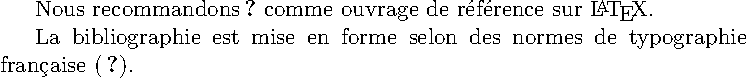
\includegraphics[width=\linewidth]{images/exemple-bibliographie-cropped-1}
    \end{framed}
    \code{xelatex} $\rightarrow$ \code{bibtex} $\rightarrow$ \code{xelatex}
    \begin{framed}
      
\includegraphics[width=\linewidth]{images/exemple-bibliographie-cropped-2}
    \end{framed}
    \code{xelatex} $\rightarrow$ \code{bibtex} $\rightarrow$ \code{xelatex} $\rightarrow$ \code{xelatex}
    \begin{framed}
      
\includegraphics[width=\linewidth]{images/exemple-bibliographie-cropped-3}
    \end{framed}
    \caption{Zone de texte du document aux diverses étapes de la
      compilation des fichiers de la
      \autoref{fig:bibliographie:bibtex:1} avec {\XeLaTeX} et
      {\BibTeX}}
    \label{fig:bibliographie:bibtex:2}
  \end{figure}
\end{exemple}

\tipbox{Aux toutes dernières étapes avant de rendre un document, s'assurer
  d'exécuter {\BibTeX} une dernière fois et de compiler avec
  pdf{\LaTeX} ou {\XeLaTeX} au moins deux fois. Le journal de la
  compilation (\emph{log file}) ne devrait pas rapporter de références
  manquantes (\emph{undefined references}).}

Les logiciels intégrés de rédaction offrent généralement des raccourcis pour exécuter la
compilation avec {\BibTeX}.
\begin{itemize}
\item Dans TeXShop, on sélectionne un autre programme dans le menu à
  côté du bouton «Composition».
\item Dans Texmaker, on choisit le programme approprié dans le menu de
  composition rapide.
\item Dans GNU~Emacs, on choisit \code{BibTeX} dans le menu
  \code{Command} ou après avoir lancé la commande
  \code{TeX-command-master} avec \code{C-c C-c}.
\end{itemize}
La \autoref{fig:bibliographie:editeurs} présente les deux premières
interfaces.

\begin{figure}
  \centering
  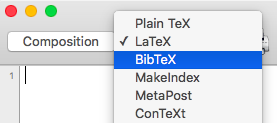
\includegraphics[height=2.2cm]{images/bibtex-texshop}
  \qquad
  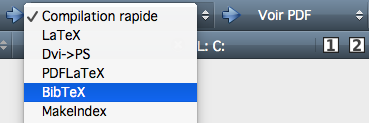
\includegraphics[height=2.2cm]{images/bibtex-texmaker}
  \caption[Interfaces de sélection du programme {\BibTeX} dans TeXShop
  et Texmaker]{%
    Interfaces de sélection du programme {\BibTeX} dans TeXShop (à
    gauche) et Texmaker (à droite)}
  \label{fig:bibliographie:editeurs}
\end{figure}

On trouvera des informations additionnelles, notamment sur des sources
de données bibliographiques et des outils de gestion des bases de
données, dans la section %
\doc[Gestion de la bibliographie]{}{https://fr.wikibooks.org/wiki/LaTeX/Gestion_de_la_bibliographie} %
de \citeauthor{wikilivres:latex}.



%%%
%%% Exercices
%%%

\section{Exercices}
\label{sec:bibliographie:exercices}

\Opensolutionfile{solutions}[solutions-bibliographie]

\begin{Filesave}{solutions}
\section*{Chapitre \ref*{chap:bibliographie}}
\addcontentsline{toc}{section}{Chapitre \protect\ref*{chap:bibliographie}}

\end{Filesave}

\begin{exercice}
  Composer des entrées de base de données pour les références
  bibliographiques suivantes.
  \begin{enumerate}
  \item \nolink{\bibentry{Mittelbach:floats:2014:nourl}}

    \emph{Astuce}: cette entrée est un article tiré d'une revue
    scientifique.

  \item \nolink{\bibentry{memoir}}

    \emph{Astuces}: traiter cette entrée comme un livre et utiliser le
    champ \code{note} pour consigner la remarque qui se trouve à la
    fin de la notice.

  \item \nolink{\bibentry{pstricks}}

    \emph{Astuces}: utiliser le type de document \code{Manual};
    attention à la casse de certains mots; on obtient le symbole {\ss}
    avec la commande \cmdprint{\ss}.
  \end{enumerate}
  \begin{sol}
    On trouve les champs obligatoires et optionnels pour chaque type
    d'entrée dans %
    \doc[Wikipedia]{}{https://fr.wikipedia.org/wiki/BibTeX}. %
    La clé est laissée vacante dans les réponses ci-dessous.
    \begin{enumerate}
    \item On utilise le type \code{Article} pour cette entrée.
\begin{lstlisting}[language=]
@Article{,
  author =  {Frank Mittelbach},
  title =   {How to Influence the Position of Float
             Environments Like Figure and Table In
             {\LaTeX}?},
  journal = {{TUG}boat},
  year =    2014,
  volume =  35,
  number =  3,
  pages =   {258-254},
  language = {english}}
\end{lstlisting}

    \item On utilise le type \code{Book} pour cette entrée.
\begin{lstlisting}[language=]
@Book{,
  author =  {Peter Wilson},
  title =   {The Memoir Class for Configurable
             Typesetting},
  publisher = {The Herries Press},
  year =     2013,
  edition =  8,
  note =    {Maintained by Lars Madsen},
  url =     {https://www.ctan.org/pkg/memoir/},
  language = {english}}
\end{lstlisting}

    \item La réponse ci-dessous contient les prénoms des auteurs,
      simplement afin d'illustrer que {\BibTeX} sait les abréger au
      moment de composer la notice bibliographique. Remarquer
      l'utilisation des accolades \verb={ }= dans le titre pour
      préserver la casse de «PSTricks» et de «PostScript».
\begin{lstlisting}[language=]
@Manual{,
  author = {Timothy {V}an Zandt and Denis Girou and
            Herbert Vo{\ss}},
  title =  {{PSTricks} --- {PostScript} Macros for
            Generic {\TeX}},
  year =   2014,
  url =    {https://www.ctan.org/pkg/pstricks-base/},
  language = {english}}
\end{lstlisting}
    \end{enumerate}
  \end{sol}
\end{exercice}

\begin{exercice}[nosol]
  Utiliser pour cet exercice le fichier
  \fichier{exercice\_gabarit.tex} ainsi que la base de données
  bibliographique crée à l'exercice précédent.
  \begin{enumerate}
  \item Créer un document simple comprenant des références à une ou
    plusieurs des entrées bibliographiques de l'exercice précédent.
    Compiler le document en suivant les étapes mentionnées à la
    \autoref{sec:bibliographie:bibtex} en utilisant tour à tour les
    styles par défaut \code{plain}, \code{unsrt}, \code{alpha} et
    \code{abbrv}.
  \item Charger dans le document le paquetage \pkg{natbib} (avant
    \pkg{babel}) et utiliser le style de bibliographie \code{francais}
    fourni par \pkg{francais-bst} (installé par défaut dans
    {\TeX}~Live). Recompiler le document et observer les différences
    par rapport aux documents produit en a).
  \end{enumerate}
\end{exercice}

\begin{exercice}[nosol]
  À partir d'un gabarit fourni avec la classe \class{ulthese},
  produire un document simple contenant une bibliographie.
\end{exercice}

\Closesolutionfile{solutions}

%%% Local Variables:
%%% mode: latex
%%% TeX-master: "formation-latex-ul"
%%% TeX-engine: xetex
%%% coding: utf-8
%%% End:

\pagestyle{plain} % en-tetes vides
% index de base
\renewcommand{\preindexhook}{%
Les entrées référencées renvoient à des numéros de verset.\\%
Les numéros de verset en \textbf{gras} indiquent la référence principale d'une entrée.%
\vskip\onelineskip\par}
\printindexv

% index d'auteurs séparé
\renewcommand{\indexname}{Index des auteurs}
\renewcommand{\preindexhook}{}
\printindexa



% \iffalse
%%% From File: toc.dtx
% \fi
%
%    \begin{macrocode}

%<*toc>
%    \end{macrocode}
%
% \subsection{������������� ������������ ������ (����������, ����������
% ��������� � �.\,�.)}
%
% \subsubsection{����� ���������}
%
% �������������� ������ ����� ���������� � ���������� ������� ����������.
% \DescribeMacro{\@postskip}\index{�������!\verb+"\"@postskip+}
%    \begin{macrocode}
\def\@postskip{\texorpdfstring{\hskip1em}{  }}
%    \end{macrocode}
% ����� ������� ����� ������������ ������ � ������� ��������.
% \DescribeMacro{\@pnumwidth}\index{�������!\verb+"\"@pnumwidth+}
%    \begin{macrocode}
\newcommand\@pnumwidth{1.55em}
%    \end{macrocode}
% ������ ������� ������.
% \DescribeMacro{\@tocrmarg}\index{�������!\verb+"\"@tocrmarg+}
%    \begin{macrocode}
\newcommand\@tocrmarg{2.55em}
%    \end{macrocode}
% ���������� ����� ��������� (�������) � ����������� ����� ��������� � �������
% (� �������� mu = 1/18 em, em --- ����� ����� |M| �������� ������).
% \DescribeMacro{\@dotsep}\index{�������!\verb+"\"@dotsep+}
%    \begin{macrocode}
\newcommand\@dotsep{4.5}
%    \end{macrocode}
% ������� ��� ���������� ���������� ����� ��������� � ������� ��������.
% \DescribeMacro{\tocfill}\index{�������!\verb*+\tocfill+}
%    \begin{macrocode}
\def\tocfill#1{%
  \leaders\hbox{$\m@th\mkern\@dotsep mu\hbox{#1}\mkern\@dotsep mu$}%
}

%    \end{macrocode}
% \subsubsection{����������}
%
% �������, ��������� ��������� � ������.
% \DescribeMacro{\tocsection}\index{�������!\verb*+\tocsection+}
%    \begin{macrocode}
\newcommand\tocsection{\chapter*{\contentsname}}

%    \end{macrocode}
% \DescribeMacro{\tableofcontents}\index{�������!\verb*+\tableofcontents+}
%    \begin{macrocode}
\newcommand\tableofcontents{%
  \if@twocolumn%
    \@restonecoltrue\onecolumn%
  \else\@restonecolfalse\fi%
  \tocsection%
  \@mkboth{\MakeUppercase\contentsname}{\MakeUppercase\contentsname}%
  \@starttoc{toc}%
  \if@restonecol\twocolumn\fi
  \clearpage
}
%    \end{macrocode}
%
% \subsubsection{������ �����������}
%
% �������, ��������� ��������� � ������.
% \DescribeMacro{\lofsection}\index{�������!\verb*+\lofsection+}
%    \begin{macrocode}
\newcommand\lofsection{\nchapter{\listfigurename}}

%    \end{macrocode}
% \DescribeMacro{\listoffigures}\index{�������!\verb*+\listoffigures+}
%    \begin{macrocode}
\newcommand\listoffigures{%
  \if@twocolumn\@restonecoltrue\onecolumn%
  \else\@restonecolfalse\fi%
  \lofsection%
  \@mkboth{\MakeUppercase\listfigurename}{\MakeUppercase\listfigurename}%
  \@starttoc{lof}%
  \if@restonecol\twocolumn\fi
}

%    \end{macrocode}
% ������ �������� ������ �����������.
%    \begin{macrocode}
\newcommand*\l@figure{\@dottedtocline{1}{1.5em}{2.3em}}

%    \end{macrocode}
%
% \subsubsection{������ ������}
%
% �������, ��������� ��������� � ������.
% \DescribeMacro{\lotsection}\index{�������!\verb*+\lotsection+}
%    \begin{macrocode}
\newcommand\lotsection{\nchapter{\listtablename}}

%    \end{macrocode}
% \DescribeMacro{\listoftables}\index{�������!\verb*+\listoftables+}
%    \begin{macrocode}
\newcommand\listoftables{%
  \if@twocolumn\@restonecoltrue\onecolumn%
  \else\@restonecolfalse\fi%
  \lotsection%
  \@mkboth{\MakeUppercase\listtablename}{\MakeUppercase\listtablename}%
  \@starttoc{lot}%
  \if@restonecol\twocolumn\fi
}

%    \end{macrocode}
% ������ �������� ������ ������.
%    \begin{macrocode}
\let\l@table\l@figure

%    \end{macrocode}
%
% \subsubsection{������������}
%
% ��������� � ��������� ����� �������������� � ������ \pkg{natbib} � �����
% � ����� \file{custom.dtx}.
% \DescribeEnv{thebibliography}\index{���������!\verb*+thebibliography+}
%    \begin{macrocode}
\newenvironment{thebibliography}[1]{}{}

%    \end{macrocode}
% �������� ������� ��� ��������� ������ ����������.
% \DescribeMacro{\bibindent}\index{���������!\verb*+\bibindent+}
%    \begin{macrocode}
\newdimen\bibindent
\setlength\bibindent{1.5em}
%    \end{macrocode}
% �������������� ������ ����� ���������� ������� �������� ������������.
% \DescribeMacro{\newblock}\index{�������!\verb*+\newblock+}
%    \begin{macrocode}
\newcommand\newblock{\hskip .11em\@plus.33em\@minus.07em}
\let\@openbib@code\@empty

%    \end{macrocode}
%
% \subsubsection{���������� ���������}
%
% �������, ��������� ��������� � ������.
% \DescribeMacro{\indexsection}\index{�������!\verb*+\indexsection+}
%    \begin{macrocode}
\providecommand\indexsection{\twocolumn[\@makeschapterhead{\indexname}]}

%    \end{macrocode}
%
% \DescribeEnv{theindex}\index{���������!\verb*+theindex+}
%    \begin{macrocode}
\newenvironment{theindex}{%
  \if@twocolumn\@restonecolfalse%
  \else\@restonecoltrue\fi%
  \columnseprule \z@
  \columnsep 35\p@
  \indexsection%
  \@mkboth{\MakeUppercase\indexname}{\MakeUppercase\indexname}%
  \thispagestyle{plain}
  \parindent\z@
  \parskip\z@ \@plus .3\p@\relax
  \let\item\@idxitem%
}{\if@restonecol\onecolumn\else\clearpage\fi}
%    \end{macrocode}
% ������ ���������.
% \DescribeMacro{\@idxitem}\index{�������!\verb+"\"@idxitem+}
% \DescribeMacro{\subitem}\index{�������!\verb*+\subitem+}
% \DescribeMacro{\subsubitem}\index{�������!\verb*+\subsubitem+}
%    \begin{macrocode}
\newcommand\@idxitem{\par\hangindent 40\p@}
\newcommand\subitem{\@idxitem \hspace*{20\p@}}
\newcommand\subsubitem{\@idxitem \hspace*{30\p@}}
%    \end{macrocode}
% ������������ ������ ����� ���������� ����������� ���������.
% \DescribeMacro{\indexspace}\index{�������!\verb*+\indexspace+}
%    \begin{macrocode}
\newcommand\indexspace{\par \vskip 10\p@ \@plus5\p@ \@minus3\p@\relax}
%</toc>
%    \end{macrocode}
 % table des matieres
\end{ltxexample}
Font partie de ce bloc: la conclusion générale, les annexes, la bibliographie, l'index et enfin la table des matières. Les en-têtes sont activées selon la logique exposée \secref{entete}.
\end{enumerate}

\subsubsection{\file{misc.tex}}

Ce fichier contient des informations diverses présentées en début de document: un avertissement, les remerciements de l'auteur et le résumé en français et anglais.

\subsubsection{\file{sommaire.tex}}

Ce fichier imprime le sommaire. Le sommaire est ici configuré pour n'afficher que les parties, titres et chapitres.

Ce fichier contient également des réglages de rendu du sommaire, qui peuvent être modifiés.

\subsubsection{\file{glossaire.tex}}

Le glossaire est géré dans le fichier \file{glossaire.tex}. Il contient la liste en vrac des termes à référencer, suivie de l'appel à la commande \cmd{printglossary}. L'option style=mcolindex permet d'imprimer le glossaire en deux colonnes. Toutes les commandes utilisées sont fournies par le package \sty{glossaries}.
\begin{ltxexample}
\<<newacronym>>{ibid.}{ibidem}
\<<newacronym>>{D.}{Recueil Dalloz}
...
\<<glsaddall>>
\<<printglossary>>[style=mcolindex]
\end{ltxexample}

\subsubsection{\file{journaux.bib}}

Ce fichier contient des chaînes de caractères \bibtex contenant des noms de revues juridiques en abrégé. Ces chaînes peuvent être utilisées dans d'autre fichiers contenant des références bibliographiques.

\subsubsection{\file{bibliographie.bib}}

Ce fichier contient une ensemble des références bibliographiques proposées à titre d'exemple. Il est chargé après le fichier \file{journaux.bib}.

\paragraph{Exemple de jurisprudence}
\label{templatejurisprudence}

Il est d'usage en droit français de grouper un arrêt (type \bibtype{jurisdiction}) avec tous les commentaires s'y référant (type \bibtype{commentary}). 

Pour lier tous ces éléments, le champ spécial \bibfield{related} dans l'entrée de type \bibtype{jurisdiction} décrivant l'arrêt:
\begin{lstlisting}[style=bibtex]{}	
@COMMENTARY{<<cass:ass:19910531:thouvenin>>,
  ...
}

@COMMENTARY{<<cass:ass:19910531:gobert>>,
  ...
}

@JURISDICTION{<<cass:ass:19910531>>,
  institution = {Cass. Ass. Pl\'en.},
  date = {1991-05-31},
  related = {<<cass:ass:19910531:thouvenin>>, <<cass:ass:19910531:gobert>>},
  keywords = {cassass}
}
\end{lstlisting}
%
Pour citer d'un seul tenant la jurisprudence couverte par ces 3 entrées, il suffit d'appeler l'entrée de type \bibtype{jurisdiction} via commande suivante depuis le corps du texte:
\begin{ltxexample}
\cite{<<cass:ass:19910531>>}
\end{ltxexample}
%

Toutes les entrées de type \bibtype{commentary} seront automatiquement accolées à la suite de l'arrêt\footnote{Attention, ce mécanisme ne fonctionne que pour des entrées de type \bibtype{commentary}.}.

On notera que l'ordre dans lequel les différentes entrées de type \bibfield{commentary} sont écrites dans le champ \bibfield{related} correspond à l'ordre d'affichage dans le document final.

On notera par ailleurs la présence d'un mot clé (ici, \enquote{cassass}) dans le champ \bibfield{keywords} du type \bibtype{jurisdiction}, pour marquer que ce groupe correspond à un arrêt rendus par la cour de cassation en assemblée plénière.

\paragraph{Exemple de code juridique}

Est ici pris en exemple le code civil. L'entrée correspondante est la suivante:
\begin{lstlisting}[style=bibtex]{}
@LEGISLATION{<<cciv>>,
  title = {Code civil},
  pagination = {section}
}
\end{lstlisting}
On notera l'utilisation de la pagination \texttt{section}, utilisée pour générer le mot-clé abrégé "art." dans la citation crée en note de bas de page.

Pour citer l'article 1642-1 du code civil, il suffit d'appeler la commande suivante depuis le corps du texte:
\begin{ltxexample}
\cite[1642-1]{<<cciv>>}
\end{ltxexample}

\paragraph{Exemple d'ouvrage dit "spécial"}

Dans beaucoup de bibliographies en droit, certains ouvrages sont qualifiés de "spéciaux", par opposition à des ouvrages dits "généraux". Cependant, cette distinction porte généralement sur le fond, et est difficilement gérable à l'aide des différents types de références proposés dans \biblatex.

Aussi, cette distinction quant au fond peut être réalisée grâce à l'utilisation d'un mot clé, par exemple "special", dans le champ \bibfield{keywords}:

\begin{ltxexample}
@BOOK{alland:dicoculturejur,
  author = {Alland, Denis and Rials, Stephane},
  title = {Dictionnaire de la culture juridique},
  date = {2003},
  publisher = {Lamy-PUF},
  keywords = {french, <<special>>}
}
\end{ltxexample}

\subsubsection{\file{bibliographie.tex}}

L'organisation de la bibliographie est gérée dans le fichier \file{bibliographie.tex}. La classification choisie est ici par pays (France et Europe) puis en 8 groupes de références: lois, rapports officiels, jurisprudence, ouvrages généraux, ouvrages spéciaux, thèses, ouvrages collectifs et enfin articles.

Le fichier est divisé en deux parties: la première définit les réglages d'organisation et la seconde imprime la bibliographie proprement dite.

\paragraph{Réglages}

Les lignes suivantes définissent des libellés de sous-bibliographies:
\begin{ltxexample}
\defbibheading{france}{\section{Droit francais}}
\defbibheading{europe}{\section{Droit europeen}}

\defbibheading{lois}{\paragraphe{Lois}}
\defbibheading{rapports}{\paragraphe{Rapports officiels}}
\defbibheading{jurisprudence}{\paragraphe{Jurisprudence}}
\defbibheading{generaux}{\paragraphe{Ouvrages generaux}}
\defbibheading{speciaux}{\paragraphe{Ouvrages speciaux}}
\defbibheading{theses}{\paragraphe{Theses}}
\defbibheading{collectifs}{\paragraphe{Ouvrages collectifs}}
\defbibheading{articles}{\paragraphe{Articles}}
\end{ltxexample}
%
On notera plus spécifiquement les libellés sous-bibliographies ci-dessous, relatives à la jurisprudence française:

\begin{ltxexample}
\defbibheading{juris:ccel}{\souspara{Conseil constitutionnel}}
\defbibheading{juris:ce}{\souspara{Conseil d'Etat}}
\defbibheading{juris:cass}{\souspara{Cour de cassation}}
\defbibheading{juris:cass:ass}{\alinea{Assemblee pleniere}}
\defbibheading{juris:cass:1civ}{\alinea{1\iere{} chambre civile}}
\defbibheading{juris:cass:2civ}{\alinea{2\ieme{} chambre civile}}
\defbibheading{juris:cass:3civ}{\alinea{3\ieme{} chambre civile}}
\defbibheading{juris:cass:com}{\alinea{Chambre commerciale}}
\defbibheading{juris:cass:soc}{\alinea{Chambre sociale}}
\defbibheading{juris:cass:crim}{\alinea{Chambre criminelle}}
\defbibheading{juris:ca}{\souspara{Cours d'appel}}
\defbibheading{juris:tgi}{\souspara{Tribunaux de grande instance}}
\defbibheading{juris:ti}{\souspara{Tribunaux d'instance}}
\end{ltxexample}
%

Chacune des ces sous-bibliographies est destinée à être peuplée d'entrées issues du fichier \file{bibliographie.bib}.

Les sous-bibliographies suivantes contiennent un unique type de référence:
\begin{itemize}
\item les lois: \bibtype{legislation}
\item la jurisprudence: \bibtype{jurisdiction} (pouvant contenant implicitement un ou plusieurs \bibtype{commentary} via le champ \bibfield{related}, voir \ref{templatejurisprudence}). Le champ \bibfield{keywords} est utilisé pour filtrer ces entrées par juridiction.
\item les thèses: \bibtype{thesis}
\end{itemize}

Les catégories suivantes comprennent plusieurs types de références:
\begin{itemize}
\item Les ouvrage dits "collectifs" comprennent les \bibtype{collection} et \bibtype{proceedings}
\item Les articles comprennent les \bibtype{article} et les contributions à des ouvrages collectifs (\bibtype{incollection} et \bibtype{inproceedings}).
\item Les ouvrage généraux et spéciaux comprennent les types \bibtype{book} et \bibtype{inbook}. La distinction entre les deux est effectuée par examen du champ \bibfield{keywords}: si la clé \texttt{special} est présente, la référence sera affichée comme ouvrage spécial, sinon comme général.
\end{itemize}

Ce choix de groupement est réalisé à l'aide des filtres ci-dessous:
\begin{ltxexample}
\defbibfilter{gen}{%
  \(\type{<<book>>} \or \type{<<inbook>>}\) \and \not \keyword{<<special>>}}
\defbibfilter{spec}{%
  \(\type{<<book>>} \or \type{<<inbook>>}\) \and \keyword{<<special>>}}
\defbibfilter{col}{\type{<<collection>>} \or \type{<<proceedings>>}}
\defbibfilter{art}{%
  \type{<<incollection>>} \or \type{<<inproceedings>>} \or \type{<<article>>}}
\end{ltxexample}
%

Pour chaque pays, le même système de groupement est utilisé. Il est combiné avec une autre clé du champ \bibfield{keywords} utilisée pour filtrer les références selon le pays.

\paragraph{Structure}

La bibliographie est imprimée grâce au jeu de commandes ci-dessous:

\begin{ltxexample}
\chapitre{Bibliographie}

\printbibheading[heading=france]

\printbibliography[heading=<<lois>>,type=<<legislation>>,keyword=<<french>>]
\printbibliography[heading=<<rapports>>,type=<<report>>,keyword=<<french>>]
\printbibheading[heading=jurisprudence]
\printbibliography[heading=<<juris:ccel>>, type=<<juridsiction>>, keyword=<<ccel>>]
\printbibliography[heading=<<juris:ce>>, type=<<juridsiction>>, keyword=<<ce>>]
\printbibheading[heading=<<juris:cass>>]
\printbibliography[heading=<<juris:cass:ass>>, type=<<juridsiction>>, keyword=<<cassass>>]
\printbibliography[heading=<<juris:cass:1civ>>, type=<<juridsiction>>, keyword=<<cass1civ>>]
\printbibliography[heading=<<juris:cass:2civ>>, type=<<juridsiction>>, keyword=<<cass2civ>>]
\printbibliography[heading=<<juris:cass:3civ>>, type=<<juridsiction>>, keyword=<<cass3civ>>]
\printbibliography[heading=<<juris:cass:com>>, type=<<juridsiction>>, keyword=<<casscom>>]
\printbibliography[heading=<<juris:cass:soc>>, type=<<juridsiction>>, keyword=<<casssoc>>]
\printbibliography[heading=<<juris:cass:crim>>, type=<<juridsiction>>, keyword=<<casscrim>>]
\printbibliography[heading=<<juris:ca>>, type=<<juridsiction>>, keyword=<<ca>>]
\printbibliography[heading=<<juris:tgi>>, type=<<juridsiction>>, keyword=<<tgi>>]
\printbibliography[heading=<<juris:ti>>, type=<<juridsiction>>, keyword=<<ti>>]
\printbibliography[heading=<<generaux>>,filter=<<gen>>,keyword=<<french>>]
\printbibliography[heading=<<speciaux>>,filter=<<spec>>,keyword=<<french>>]
\printbibliography[heading=<<collectifs>>,filter=<<col>>,keyword=<<french>>]
\printbibliography[heading=<<theses>>,type=<<thesis>>,keyword=<<french>>]
\printbibliography[heading=<<articles>>,filter=<<art>>,keyword=<<french>>]

\printbibheading[heading=europe]

\printbibliography[heading=<<lois>>,type=<<legislation>>,keyword=<<ue>>]
\printbibliography[heading=<<rapports>>,type=<<report>>,keyword=<<ue>>]
\printbibliography[heading=<<jurisprudence>>,type=<<juridsiction>>,keyword=<<ue>>]
\printbibliography[heading=<<generaux>>,filter=<<gen>>,keyword=<<ue>>]
\printbibliography[heading=<<speciaux>>,filter=<<spec>>,keyword=<<ue>>]
\printbibliography[heading=<<collectifs>>,filter=<<col>>,keyword=<<ue>>]
\printbibliography[heading=<<theses>>,type=<<thesis>>,keyword=<<ue>>]
\printbibliography[heading=<<articles>>,filter=<<art>>,keyword=<<ue>>]
\end{ltxexample}
%

Deux commandes fournies par le package \biblatex sont utilisées pour imprimer la bibliographie: \cmd{printbibliography} et \cmd{printbibheading}.

La commande \cmd{printbibheading} est relativement simple: elle sert uniquement à imprimer un titre de bibliographie, sans contenu.

la commande \cmd{printbibliography} imprime un ensemble de références bibliographiques issues des fichiers qui ont été référencés en préambule du document au moyen de la commande \cmd{addbibresource} (voir le fichier maître \file{main.tex}). La commande \cmd{printbibliography} sélectionne des références sur la base de critères de sélection passés en arguments. Comme le montre les lignes ci-dessus, les options \texttt{heading}, \texttt{filter}, \texttt{type} et \texttt{keyword} sont utilisées comme critères de sélection.

On notera en particulier que le champ \bibfield{keywords} est utilisé de façon à filter les références de type \bibtype{jurisdiction} par juridictions. Le tableau \ref{clesjuridictions} propose des exemples de mots-clés pour la plupart des juridictions françaises. Bien entendu, ces mots-clés sont à la discrétion du rédacteur.

\begin{table}
\tablesetup
\begin{tabularx}{\textwidth}{@{}@{}p{200pt}>{\ttfamily}X@{}}
\toprule
\multicolumn{1}{@{}H}{Juridiction} &
\multicolumn{1}{@{}H}{mot-clé à inclure au champ \bibfield{keywords}} \\
\cmidrule(r){1-1}\cmidrule(r){2-2}
Conseil constitutionnel & cc \\
Conseil d'État & ce \\
Cour de cassation (générique) & cass \\
Cour de cassation en assemblée plénière & cassass \\
1\iere{} chambre civile & cass1civ \\
2\ieme{} chambre civile & cass2civ \\
3\ieme{} chambre civile & cass3civ \\
Chambre criminelle & casscrim \\
Chambre sociale & casssoc \\
Chambre commerciale & casscom \\
Tribunal de grande instance & tgi \\
Tribunal d'instance & ti \\

\bottomrule
\end{tabularx}
\caption{Mots-clés de filtrage par juridiction française}
\label{clesjuridictions}
\end{table}

\subsubsection{\file{index.tex}}

Ce fichier imprime l'index par versets de base et l'index d'auteurs par verset, au moyen des commandes suivantes.
\begin{ltxexample}
\printindexv
\printindexa
\end{ltxexample}

\subsubsection{\file{toc.tex}}

Ce fichier imprime la table des matières. Contrairement au sommaire, la table des matière affiche tous les niveaux de subdivisions fournis par la classe \sty{\classname}, sauf les versets.

Ce fichier contient également des réglages de rendu de la table des matières, qui peuvent être modifiés.

\subsubsection{\file{main.pdf}}

Ce fichier est le résultat de la compilation du projet complet. Tous les liens actifs dans le document sont encadrés de rouge. Ces cadres disparaissent lors d'une impression papier.

Voir \secref{compilation} pour plus de détails concernant l'étape de compilation.

\subsection{Compilation}
\label{compilation}

\subsubsection{En ligne de commande}

Voici la séquence de compilation minimale à effectuer sur le fichier principal \file{main.tex} pour produire le fichier \file{main.pdf}:

\begin{lstlisting}[style=plain]{}
pdflatex main.tex
makeindex -s index.ist -o index.idx index.ind
makeindex -s auteurs.ist -o auteurs.idx auteurs.ind
makeglossaries main.glo
biber main.bcf
pdflatex main.tex
pdflatex main.tex
\end{lstlisting}
%
Plusieurs passes sur le programme \texttt{pdflatex} sont nécessaires pour résoudre les problèmes de références croisées.

Le programme \texttt{makeindex} est à appeler deux fois, pour l'index de base et l'index d'auteurs. Les fichiers d'extension \file{.ist} sont des fichiers de style passés en paramètre de \texttt{makeindex}; ils sont créés à la première passe de pdflatex si absents.

Le programme \texttt{makeglossaries} est un script Perl qui génère le glossaire. Il nécessite l'installation préalable d'une distribution Perl.

Le programme \texttt{\biber} participe à la génération de la bibliographie. Il doit être appelé une fois en lieu et place de \bibtex.

\subsubsection{Avec Latexmk}

Latexmk\fnurl{http://www.phys.psu.edu/~collins/software/latexmk-jcc/} est un programme qui gère de manière interne les étapes intermédiaires de compilation décrites précédemment. Dans un unique appel à latexmk, latex, makeindex et biber sont appelés autant de fois que nécessaire afin de produire un fichier PDF:

\begin{lstlisting}[style=plain]{}
latexmk main.tex
\end{lstlisting}
%

Pour effacer tous les fichiers générés au cours de la compilation sauf le PDF final, il suffit d'appeler le programme avec l'option -c.

\begin{lstlisting}[style=plain]{}
latexmk -c
\end{lstlisting}
%

Le fichier \file{latexmkrc} contient des paramètres permettant d'exécuter automatiquement la séquence manuelle définie dans la section précédente; sa présence dans le répertoire de travail est donc \emph{indispensable}.

%\subsection{Adaptation de l'exemple}
%TODO: finir cette section
%UTF8

\section{Recommandations et astuces}
\label{astuces}

Cette partie a pour objectif de recenser un certain nombre d'astuces utiles pour le rédacteur.

\subsection{Le choix des logiciels}

\subsubsection{L'éditeur \latex}

Beaucoup d'éditeurs \latex gratuits existent, avec des approches différentes.

\texttt{Texmaker} offre un bon compromis entre simplicité et puissance:
\begin{itemize}
\item il est disponible sous Linux, Mac et Windows
\item l'interface graphique n'est pas surchargées de boutons inutiles
\item on peut utiliser LatexMk pour la compilation (très fortement recommandé!)
\item prévisualisation simple et efficace du PDF généré, avec changements récents apparaissant brièvement en rouge à l'ouverture du PDF
\item bascule très simple depuis un endroit du PDF vers le code source \latex correspondant, et vice-versa. Ceci  est particulièrement efficace pour corriger des coquilles à la lecture du PDF\fnurl{http://itexmac.sourceforge.net/SyncTeX.html}.
\end{itemize}

\subsubsection{Le gestionnaire de bibiographie}

Éditer à la main son ou ses fichiers \file{.bib} est possible, mais s'avère fastidieux et sensible aux erreurs. Il est donc conseillé de passer par un gestionnaire de bibliographie, qui présentera le contenu du fichier \file{.bib} sous la forme d'une base de donnée.

Attention, \biblatex est une extension relativement récente de \bibtex, que beaucoup de gestionnaires de bibliographies ne prennent pas en charge.

Le logiciel Jabref est très fortement recommandé\fnurl{http://jabref.sourceforge.net}. Il présente beaucoup d'avantages:
\begin{itemize}
\item il est disponible sous Linux, Mac et Windows
\item il dispose d'un mode "bibatex" (à activer)
\item il est possible d'ajouter facilement des types d'entrées non standards (comme \bibtype{legislation}, \bibtype{jurisdiction} ou \bibtype{commentary}) 
\end{itemize}

\subsection{Conventions de nommage}

Il est très fortement recommandé de suivre une certaine discipline pour le nommage de certaines clés.

\subsubsection{Clés \bibtex}

Chaque référence bibliographique comporte une clé \bibtex devant être absolument unique. Cette clé est passée en paramètre de la commande \cmd{cite} dans le corps du texte, pour créer une citation de cette entrée en bas de page.

Pour les références classiques, une clé formée par des abbréviations de nom d'auteur, de titre et l'année de publication est efficace. Pour éviter les incertitudes, tout est mis en minuscules et |:| est utilisé comme caractère séparateur.

Exemple: 
\begin{lstlisting}[style=bibtex]{}
@THESIS{<<baillon:famillemort:2006>>,
  author = {Baillon-Wirtz, Nathalie},
  title = {La famille et la mort},
  date = {2006},
}
\end{lstlisting}

Pour les références jurisprudentielles, on peut opter pour une forme différente:
\begin{itemize}
\item Pour les \bibtype{jurisdiction}, on peut utiliser le nom de l'institution suivi de la date précise de l'arrêt au format YYYYMMDD;
\item Pour les \bibtype{commentary}, même chose, en indiquant en plus le nom de l'auteur principal du commentaire d'arrêt;
\end{itemize}

Exemple:
\begin{lstlisting}[style=bibtex]{}
@COMMENTARY{<<cass1civ:20100622:dupond>>,
  editor = {Dupond, Albert},
  ...
}

@JURISDICTION{<<cass1civ:20100622>>,
  institution = {Cass 1\iere{} civ.},
  eventdate = {2010-06-22},
  related = {cass1civ:20100622:dupond}
}

\end{lstlisting}

\subsubsection{Clés du champ \texttt{keywords}}

Ce champ est utilisé pour la sélection d'entrées particulières lors de l'invocation de la commande \cmd{printbibliography}.

Des clés courtes et explicites sont à préférer.

\subsubsection{Références croisées}

Pour les références croisées, ne pas hésiter à entrer des clés suffisamment précises pour ne pas créer de doublons. 

\subsection{Usage des guillemets}

\begin{ltxsyntax}

\cmditem{enquote}{texte}
\cmditem{enquote*}{texte}
\label{guillemets}

Les règles de typographie française sont très strictes. Elles imposent l'utilisation de caractères spécifiques pour les guillemets: \enquote{} dans un contexte habituel, et \enquote*{ } à l'intérieur d'autres guillemets. La commande \cmd{enquote} du package \sty{csquotes} permet de gérer ces deux niveaux en fonction du contexte. La variante étoilée permet de forcer l'affichages des guillemets de second niveau \enquote*{ }.

Voici une exemple où les deux niveaux sont utilisés, et le rendu obtenu après compilation:
\begin{ltxexample}
\enquote{Il m'a dit: \enquote{tu...}}
\end{ltxexample}
\enquote{Il m'a dit: \enquote{tu...}}\\

L'utilisation du guillemet anglais |"| est à proscrire. La commande \cmd{enquote} est la seule capable de gérer les deux niveaux de guillemets français; les commandes \cmd{og} et \cmd{fg} proposées par le package \sty{babel} ne gèrent pas les guillemets de second niveau et sont donc insuffisants.

\end{ltxsyntax}

\subsection{Usages particuliers de \biblatex}

Les fonctionnalités du package \biblatex sont pour la plupart faciles à prendre en main, pour peu que l'on s'attaque à sa documentation assez titanesque. Toutefois, certains d'entre eux doivent être utilisés de manière spéciale en français.

Sont donc ici répertoriés certaines options de ce package particulièrement intéressantes, et certaines finesses d'utilisation des champs de références bibliographiques.

\subsubsection{Usages particuliers de champs}

\paragraph{Noms complexes à particule}

Pour rappel, les champs relatifs à des noms d'auteur, tels que le champ \bibfield{author}, peuvent contenir une liste d'éléments distincts délimités à l'aide du délimiteur \texttt{and}. Chaque élément est décomposé à la compilation en quatre parties: prénom, particule (de, von, of), nom de famille, et suffixe (junior, senior, \dots).

Or, certains noms de famille complexes posent des problèmes de rendu car ils ne sont pas facilement décomposables en ces 4 parties.

Pour prévenir ce genre de problème, une paire d'accolades supplémentaires et/ou des espaces insécables peuvent être insérées dans la définition des champs \bibfield{author} et \bibfield{editor}. En voici un exemple:

\begin{lstlisting}[style=bibtex]{}
author = {<<{Delaisi de Parseval}>>, Genevieve and Depadt-Sebag, Valerie},
\end{lstlisting}

\paragraph{Groupes d'auteurs/rédacteurs}

Les champs \bibfield{author} or \bibfield{editor} peuvent contenir des noms de groupes lorsque cela est nécessaire\footnote{Les noms de groupes sont particulièrement fréquents dans les rapports officiels.}. Pour éviter que ces groupes soient traités comme des noms de personnes (prénom, nom, etc), une paire supplémentaire d'accolades est nécessaire. Les champs optionnels \bibfield{shortauthor} et \bibfield{shorteditor} sont destinés à contenir des noms abrégés pour usage dans les citations.

\begin{lstlisting}[style=bibtex]{}
editor       = {<<{Comit\'e Consultatif National d'\'Ethique}>>
                and Dupont, Marcel},
shorteditor  = {CCNE and Dupont, Marcel},
\end{lstlisting}

\paragraph{Titres d'ouvrages}

Les exemples suivants montrent comment gérer les titres dans différents contextes.
Voici un premier exemple avec un ouvrage de 5 volumes:

\begin{lstlisting}[style=bibtex]{}
@Book{works,
  author     = {Shakespeare, William},
  title      = {Collected Works},
  volumes    = {5},
  ...
\end{lstlisting}
%
Chaque volume d'un ouvrage en plusieurs volumes ont généralement un titre spécifique. Supposons que le quatrième volume de l'ouvrage \emph{Collected Works} inclut les sonnets de Shakespeare et que l'on souhaite faire référence à ce volume seul:

\begin{lstlisting}[style=bibtex]{}
@Book{works4,
  author     = {Shakespeare, William},
  maintitle  = {Collected Works},
  title      = {Sonnets},
  volume     = {4},
  ...
\end{lstlisting}
%
Si les différents volumes sont sans titre, utiliser simplement le champ \bibfield{title} et indiquer le numéro de volume:

\begin{lstlisting}[style=bibtex]{}
@Book{works4,
  author     = {Shakespeare, William},
  title      = {Collected Works},
  volume     = {4},
  ...
\end{lstlisting}
%
Dans l'exemple suivant, on souhaite faire référence à la partie titrée d'une volume ayant également son titre propre:

\begin{lstlisting}[style=bibtex]{}
@InBook{lear,
  author     = {Shakespeare, William},
  bookauthor = {Shakespeare, William},
  maintitle  = {Collected Works},
  booktitle  = {Tragedies},
  title      = {King Lear},
  volume     = {1},
  pages      = {53-159},
  ...
\end{lstlisting}

\paragraph{Rôles rédactionnels}
\label{roles}

Le rôle joué par un rédacteur dans les champs dédiés (\ie \bibfield{editor}, \bibfield{editora}, \bibfield{editorb}, \bibfield{editorc}) peut être spécifié dans les champs \bibfield{editor...type} correspondants. 

Les rôles suivantes sont supportés par le style \bibstylename:

\begin{marglist}
\setlength{\itemsep}{0pt}
\item[editor] la personne ayant dirigé la rédaction de l'ouvrage (nom précédé de "sous la dir. de"). Il s'agit du rôle le plus répandu et est la valeur par défaut.
\item[commentator] Auteur d'une commentaire (nom précédé de "comm.").
\item[annotator] Auteur d'une note (nom précédé de "note.").
\item[observator] Auteur d'une observation (nom précédé de "obs.")
\item[chronicler] Auteur d'une chronique (nom précédé de "chron.")
\item[author] Auteur (nom précédé de "par ").
\end{marglist}
%
Voici l'exemple d'un commentaire d'arrêt la personne indiquée en \bibfield{editor} occupe le rôle d'observateur:

\begin{lstlisting}[style=bibtex]{}
@COMMENTARY{...,
  editor      = {Dupond, Marcel},
  editortype  = {<<observator>>},
  ...
\end{lstlisting}
%
L'exemple ci-dessous présente un commentaire d'arrêt dans lequel plusieurs rédacteurs on joué un rôle spécifique:

\begin{lstlisting}[style=bibtex]{}
@COMMENTARY{...
  editor = {Bernard, J},
  editortype = {<<commentator>>},
  editora = {Terr\'e, F.},
  editoratype = {<<annotator>>},
  afterword = {Dontewille}
  ...
}
\end{lstlisting}
%
On notera au passage que le champ \bibfield{afterword} (tout comme \bibfield{foreword}) suit une logique différente.

\paragraph{Dates}
\label{dates}

\begin{table}
\tablesetup
\begin{tabularx}{\textwidth}{@{}>{\ttfamily}llX@{}}
\toprule
\multicolumn{1}{H}{Valeur du champ date} &
\multicolumn{1}{H}{Rendu obtenu} \\
\cmidrule{1-1}\cmidrule(l){2-2}
1850			& 1850 \\
1997/			& 1997-- \\
1967-02			& fév. 1967 \\
2009-01-31		& 31 jan. 2009 \\
1988/1992		& 1988--1992 \\
2002-01/2002-02		& jan. 2002--fév. 2002 \\
1995-03-30/1995-04-05	& 30 Mar. 1995--5 avr. 1995 \\
\bottomrule
\end{tabularx}
\caption{Formats de dates}
\label{bib_use_tab1}
\end{table}

Les champs \bibfield{date} et \bibfield{eventdate} requièrent un format \texttt{yyyy-mm-dd}. Les intervalles de dates requièrement le format \texttt{yyyy-mm-dd\slash yyyy-mm-dd}. Une date de commencement peut être donnée en omettant la date de fin après le slash de séparation (\texttt{yyyy/}). Des exemples sont données \tabref{bib_use_tab1}.

\paragraph{Pagination}
\label{bib_use_pag}

Lorsque un numéro de page ou un intervalle de pages est indiqué dans le champ \bibfield{pages} (ou dans l'argument \prm{postnote} d'une commande de citation), le préfixe "p." est automatiquement ajouté en amont de ce numéro ou intervalle.

Or, certains ouvrages optent pour un système de pagination différent: numéro de paragraphe, de ligne, etc. Les champs \bibfield{pagination} et \bibfield{bookpagination} permet de modifier le comportement par défaut. Pour exemple, considérons l'entrée suivante:

\begin{lstlisting}[style=bibtex]{}
@InBook{..,
  title          = {...},
  pagination     = {verse},
  booktitle      = {...},
  bookpagination = {page},
  pages          = {53--65},
  ...
\end{lstlisting}
%
Le champ \bibfield{bookpagination} affecte le rendu des champs \bibfield{pages} et \bibfield{pagetotal} dans la liste des références bibliographiques. Le champ \bibfield{pagination}, lui, affecte le rendu des informations de pages passée en argument \prm{postnote} des commandes de citation. Lorsque l'un ou l'autre de ces deux champs est laissé vide, la pagination \texttt{page} est appliquée par défaut.

Dans l'exemple ci-dessus, le contenu du champ \bibfield{pages} apparaîtra sous la forme "p.~53--65" (le champ \bibfield{bookpagination} aurait pu être laissé vide, la pagination \texttt{page} étant celle par défaut). Dans une citation du style |\cite[17]{key}|, la postnote sera sous la forme "v.~17".

Les valeurs autorisées pour les champs \bibfield{pagination} and \bibfield{bookpagination} sont: \texttt{page}, \texttt{column}, \texttt{line}, \texttt{verse}, \texttt{section}, \texttt{paragraph} et \texttt{article}. La valeur "\texttt{none}" désactive tout préfixe devant l'information de page.

\subsubsection{Présentation en sous-bibliographies}

En droit, il est d'usage de subdiviser une bibliographie selon certains critères. etc. Ceci est réalisable grace aux arguments passés à la commande \cmd{printbibliography}, décrite précédemment.

Dans l'exemple ci-dessous, on souhaite divider un chapitre bibliographie en deux sections, l'une dédiée au droit français, l'autre au droit européen. Chaque section sera elle-même décomposée en paragraphes, contenant chacun un type de référence.

On commence par définier des titres de paragraphe pour chaque type d'entrée:

\begin{lstlisting}[style=latex]{}
\defbibheading{lois}{\paragraphe{Lois}}
\defbibheading{rapports}{\paragraphe{Rapports officiels}}
...
\end{lstlisting}
%

L'attribution des références dans les deux sections majeures est effectuée à l'aide du champ \bibfield{keywords}: toutes les entrées contenant le mot clé \texttt{french} seront imprimées dans la section française, celles contenant \texttt{eu} dans la section européenne:

\begin{lstlisting}[style=latex]{}
\section{Droit interne}
\printbibliography[<<heading=lois>>,type=legislation,<<keyword=french>>]
\printbibliography[<<heading=rapports>>,type=report,<<keyword=french>>]
...

\section{Droit de l'Europe}
\printbibliography[<<heading=lois>>,type=legislation,<<keyword=eu>>]
\printbibliography[<<heading=rapports>>,type=report,<<keyword=eu>>]
...
\end{lstlisting}
%

\subsubsection{Numéros de page dans les citations}
\label{use_cav_pag}

Si l'argument \prm{postnote} d'une commande de citation est un numéro de page ou un intervalle de pages, le préfixe de pagination est généré (voir \secref{bib_use_pag} sur la pagination). Voici quelques exemples de \prm{postnote} reconnus comme des informations de pages:

\begin{lstlisting}[style=latex]{}
\cite[<<25>>]{key}
\cite[<<vii>>]{key}
\cite[<<XIV>>]{key}
\cite[<<34--38>>]{key}
\cite[<<iv--x>>]{key}
\cite[<<185/86>>]{key}
\cite[<<XI \& XV>>]{key}
\cite[<<3, 5, 7>>]{key}
\cite[<<vii--x; 5, 7>>]{key}
\end{lstlisting}
%

Si la postnote ne contient pas exactement une information purement numérique, elle est imprimée telle quelle. Aussi, il est possible d'écrire le préfixe de pagination manuellement:

\begin{lstlisting}[style=latex]{}
\cite[<<p.~5>>]{key}
\end{lstlisting}
%
Il est possible de supprimer le préfixe de pagination référence par référence dans les citations, en affectant au champ \bibfield{pagination} la valeur "\texttt{none}"; voir \secref{bib_use_pag} pour plsus de détails.

\subsubsection{Tri manuel des références bibliographiques}
\label{use_srt}

Le classement des références bibliographiques actif par défaut dans le style bibliographique \sty{\bibstylename} est le classement \texttt{nyt} se fait d'abord par nom d'auteur, puis par date, enfin par titre.

Cependant, il s'avère que ce système de classement n'est pas le plus adapté dans certains cas.

Il est possible d'influer sur le classement automatique auteur/année/titre grâce au champ spécial \bibfield{presort} dont la format attendu est une lettre alphabétique. Les entrées affublées de la valeur "\texttt{a}" seront imprimées en premier, celles ayant la valeur "\texttt{z}" en dernier. Ce tri peut être affiné en utilisant un deuxième caractère: la valeur "\texttt{aa}" est imprimée en premier, suivi de "\texttt{ab}", "\texttt{ac}", etc. Les entrées dont le champ \bibfield{presort} est laissé vide sont implicitement classées à la valeur "\texttt{mm}".

Prenons un exemple concret de 3 entrées \texttt{ref1}, \texttt{ref1} et\texttt{ref3}, que l'on souhaite afficher dans cet ordre dans la bibliographie, quels que sont leur auteur, titre et année. Le champ presort peut être utilisé comme suit:

\begin{lstlisting}[style=bibtex]{}
@Book{ref1,
  presort = {<<a>>},
  ...
}

@Book{ref2,
  presort = {<<b>>},
  ...
}

@Book{ref3,
  % champ presort indefini => valeur implicite <<"m">>
  ...
}
\end{lstlisting}
%

Le tri manuel des références est particulièrement adapté aux références jurisprudentielles, que l'on classe généralement par importance de juridiction. On définira alors une valeur explicite au champ \bibfield{presort} des entrées de type \bibtype{jurisdiction}.



% TODO
%Erreurs de compilation fréquentes


%\section{Guide du programmeur}
%
%Cette partie s'addresse aux personnes souhaitant comprendre plus en détail le fonctionnement de la classe \sty{\classname} et du style bibliographique afin de l'adapter à des besoins spécifiques. De bonnes connaissances de \latex sont souhaitables avant d'aller plus loin.
%
%\subsection{Style des niveaux hiérarchiques}
%
%classe \sty{\classname}.
%
%\subsection{Style de la bibliographie}
%
%Cette partie s'addresse aux personnes souhaitant modifier le code du style bibliographique. 
%la lecture de la documentation complète du package Biblatex absolument indispensable.
%
%Deux fichiers de styles sont disponibles:
%bbx: style de la bibliographie présentée en fin de document
%cbx: styles des citations (en note de bas de page).
%
%Le fonctionnement général est le suivant: 
%
%pour chaque type d'entrée bibliographique, le fichier bbx définit un "driver". Ce driver expose les champs supportés par le type d'entrée, leur ordre et leur format (entre guillements, en italique...) dans la bibliographie.
%
%La présentation des références dans une citation en bas de page présente des variantes.
%
%l'ordre et le style de pésentatun "driver" est défini


\end{document}

